% !TeX program = xelatex
% ============================================================================
%  2026 年高教社杯全国大学生数学建模竞赛  C 题
%  微网与外部电网电力调控策略
%
%  全文：摘要 + §1 问题重述 ~ §8 参考文献 + 附录
%  编译：xelatex paper.tex   （或 latexmk -xelatex paper.tex）
%  依赖：cumcmthesis.cls（同目录）、figures/*.png
% ============================================================================
% withoutpreface：去掉承诺书与编号页，正文自摘要起排（电子版提交用）
\documentclass[withoutpreface]{cumcmthesis}

% 代码清单用覆盖较广的等宽字体（Latin Ext-A、希腊字母、上下标、箭头符号）
\setmonofont{Consolas}[Scale=0.92]

\usepackage{tikz}
\usetikzlibrary{arrows.meta,positioning,shapes.geometric,calc,fit,backgrounds}
\usepackage{amsmath}
\usepackage{booktabs}
\usepackage{multirow}
\usepackage{array}
\usepackage[section]{placeins}   % 浮动体不得越出所在章节

% 中文强调改用加粗：ctex 默认把中文 \emph 渲染成下划线，本文不使用下划线
\renewcommand{\emph}[1]{\textbf{#1}}

% 附录代码的注释里含希腊字母、上下标与数学符号，等宽字体无这些字形；
% 交给中文字体渲染，避免 "Missing character"。
\xeCJKDeclareCharClass{CJK}{"00A0 -> "00FF,   % Latin-1 补充（× · ± 等）
                            "0100 -> "017F,   % Latin Extended-A（ĉ ĝ）
                            "0300 -> "036F,   % 组合附加符号
                            "0391 -> "03C9,   % 希腊字母
                            "2000 -> "206F,   % 通用标点（… 等）
                            "2070 -> "209F,   % 上标与下标
                            "2190 -> "21FF,   % 箭头
                            "2200 -> "22FF,   % 数学运算符
                            "2500 -> "257F,   % 制表符号
                            "25A0 -> "25FF,   % 几何图形（★ 等）
                            "27F0 -> "27FF}   % 补充箭头（⟹ ⟺）

% ---- TikZ 统一风格 ----
\tikzset{
  box/.style   = {rectangle, rounded corners=2pt, draw=black!65, fill=blue!5,
                  line width=0.5pt, minimum height=0.70cm, minimum width=1.8cm,
                  align=center, font=\footnotesize, inner sep=3pt},
  databox/.style = {box, fill=orange!10},
  resbox/.style  = {box, fill=green!10},
  warnbox/.style = {box, fill=red!8},
  ar/.style    = {-{Stealth[length=2.2mm]}, draw=black!70, line width=0.6pt},
  dar/.style   = {ar, dashed}
}

\newcommand{\hd}[1]{\textbf{#1}}
\renewcommand{\arraystretch}{1.02}

% 表名与图名用小五（9pt）；正文保持模板默认的小四（12pt）。
% 模板在 \captionsetup[figure]/[table] 里写了 font={song,minusfour,bf}，
% 故须按环境分别覆盖，全局 \captionsetup{font=} 会被其覆盖。
\DeclareCaptionFont{xiaowu}{\zihao{-5}}
\DeclareCaptionFont{songwu}{\songti\zihao{-5}}
\captionsetup[figure]{font={songwu,bf}}
\captionsetup[table]{font={songwu,bf}}
% 行距收紧，为全文留出页数
\renewcommand{\baselinestretch}{1.22}
% 公式上下留白与多行公式行距
\setlength{\abovedisplayskip}{4pt plus 2pt minus 1pt}
\setlength{\belowdisplayskip}{4pt plus 2pt minus 1pt}
\setlength{\abovedisplayshortskip}{2pt}
\setlength{\belowdisplayshortskip}{2pt}
\setlength{\jot}{1.5pt}

% ============================================================================
\title{基于分位对冲与场景化日内调整的微网两阶段购电策略优化模型}
\tihao{C}
\baominghao{2026C-XXXX}
\schoolname{XX 大学}
\membera{队员 A}
\memberb{队员 B}
\memberc{队员 C}
\supervisor{指导教师}
\yearinput{2026}
\monthinput{9}
\dayinput{XX}

\begin{document}


\maketitle

% ===================================================================== 摘要
\begin{abstract}
微网在低电价时段购电存入储能、在高峰时段放电供负载，可降低购电费用；光伏出力与
电价的随机性又使买多少电成为带对冲性质的决策问题。本文围绕计划、调整与紧急购电
三层电价结构，对四个子问题建立了递进式的购电策略模型。

\textbf{问题一}中电价、负载与光伏全天已知，本质是储能套利下的\textbf{确定性线性规划}：
以 144 个 10 分钟区间的购电量、充放电功率与储电量为决策变量，用 HiGHS 求解。
全天购电量 \textbf{59\,482.70 kWh}、购电费 \textbf{35\,126.95 元}，
弃光为零，储电量全程满足安全区间且首末相等。

\textbf{问题二}引入负载与光伏的逐日变化及 5 倍价紧急购电。本文先划清时间边界——0:00
只承诺计划购电量，充放电与紧急购电皆是实时追索量；再以可交付充电下确界构造覆盖率
取 1 的计划，按逐槽递推的因果策略执行。情景集由\textbf{低需求日分组}给出：数据显示
区分各日的不是星期而是用电水平，低需求日（周五、周六）的日均净负荷仅为其余五天的
约三分之一，据此取回看 6 天内的同组历史日（无前视），使全年费用较按星期取样下降
\textbf{8.51\%}。全年总购电费 \textbf{13\,846\,553 元}（其中紧急购电费 619\,617 元）。

\textbf{问题三}加入 6:00/12:00/18:00 三档预报与调整通道。附件 3 只给整点预报，
本文按其“整点时刻值”的原义\textbf{线性插值}到 10 分钟粒度，避免分段常数削平正午峰值。
按计划量全额付费口径，模型组织为\textbf{计划、调整、执行与结算四层因果结构}：
计划层充放电取\textbf{逐情景追索变量}、购电按题面字面读法\textbf{不设上界}，并由该口径
推出\textbf{调整只允许上调、违约费恒为零}（实测 0 元）。全年总购电费 \textbf{13\,630\,568 元}，
高出同口径完美预见下界 \textbf{$11.46\%$}；消融显示日内调整通道值 105.96 万元、
水平校正 8.04 万元、低需求日分组 61.04 万元。

\textbf{问题四}换用附件 4 的逐日逐槽实际电价。方差分解显示日内形状占 \textbf{$84.6\%$}、
日水平因子仅占 \textbf{$9.2\%$}，而四项收费同为电价的倍数、日水平又只是全天均匀平移，
故电价的整体水平\textbf{只改变账单、不改变决策}——实测换价后各决策量逐元素不变。

灵敏度分析表明：模型对分位参数与电价水平都不敏感（分位平台总费极差 $0.017\%$，
价格 $\pm30\%$ 共 13 档下策略逐元素不变），而对预报档位与购电上界的\emph{读法}较敏感，
两种读法须分层陈述。

本文的创新点在于：（1）以\textbf{低需求日分组}构造情景集：由暖机期日均净负荷推出
低需求日、取同组历史日，全程无前视，显著优于按星期取样与不分组；（2）把附件 3 的
整点预报按“整点时刻值”的原义\textbf{线性插值}到 10 分钟粒度，正午净需求预报误差由
分段常数的 867 kW 降至 \textbf{524 kW}；（3）把三档价差归结为\textbf{分块分位对冲}
规则，并给出该分位只能扫描、不能由静态报童临界比推出的实测证据；（4）以
\textbf{可交付充电下确界}统一规划层与执行层的储能物理。

\textbf{关键词}：微网购电策略\quad 分位数对冲\quad 两阶段随机优化\quad 储能调度
\end{abstract}

% ===================================================================== §1
\section{问题重述}

\subsection{问题背景}

随着分布式光伏在配电网中的渗透率不断提高，如何就地消纳光伏发电、减少对大电网的
依赖，成为能源系统运行中的一个现实问题。微网正是为解决这一问题而发展起来的小型
发用电系统，它由分布式电源、储能装置和本地负载构成；非孤岛运行的微网还与外部电网
相连，可以在电价较低或分布式能源有剩余电量的时段为储能设备充电，并在电价较高的
时段释放电能，以获得经济上的收益。

在本题的场景中，微网需要利用小区负载、光伏发电量和储能设备当前储电量等数据，
在每天 0:00 给出当天的计划购电量与储能设备的充放电量，使供给的电力既能满足小区
负载，又尽可能节省购电费用。问题的难点有两方面：一是光伏出力和负载都具有随机性，
当天的实际情况未必与预期一致；二是储能设备的容量、功率与效率都受硬约束，购电
决策必须在买少了须按高价补购、买多了用不掉也须照付之间权衡。

附录 1 给出储能设备的参数：最大容量 12000 kWh，最大充放电功率 5000 kW，
2025 年 1 月 1 日 0:00 的起始电量为 6000 kWh，运行中电量须保持在 1200 至 10800 kWh
之间，充放电效率为 90\%。题目提供四份数据附件：附件 1 是某天的电价、小区负载与
光伏发电预测功率，供问题一使用；附件 2 是 2025 年全年逐 10 分钟的负载与光伏实际
功率；附件 3 是全年每天 0:00、6:00、12:00、18:00 发布的未来 24 小时整点光伏功率
预报；附件 4 是全年逐 10 分钟的电价。

\subsection{问题提出}

问题一处理最理想的情形：电价与小区负载每天相同，光伏出力也有逐 10 分钟的预测
数据，全部输入均为已知。要求在微网供给的电能不低于小区负载、储能设备在 0:00 与
24:00 的储电量相同的条件下，建立每天 0:00 制定当天计划购电策略的数学模型，
并给出具体的计划购电策略。

问题二放松了负载与光伏每天相同这一条件。电价仍不变，但负载与光伏逐日逐时段
变化；若微网供给的电能低于负载，缺口部分需按交易时刻电价的 5 倍紧急购电，而除
紧急购电费用外，其余时段的购电费用均按计划购电量结算。要求建立每天 0:00 制定
当天计划购电策略的数学模型。

问题三进一步引入预报信息。每天 0:00、6:00、12:00、18:00 可获得未来 24 小时整点的
光伏功率预报，因此除在 0:00 制定计划外，还可在其余三个时刻依据新预报调整计划。
计划量高于调整量的部分按交易时刻电价的 50\% 计违约金，调整量高于计划量的部分按
1.5 倍计价，总费用由计划购电费、紧急购电费与调整购电量的相关费用构成。要求建立
当天购电策略的数学模型，并分析是否需要引入其他时刻的预报。

问题四把电价也改为实时波动，要求针对波动电价建立微网当天购电策略的数学模型，
并依据附件 2、附件 3、附件 4 重新计算问题二与问题三。

% ===================================================================== §2
\section{问题分析}

\subsection{总体思路}

四个子问题共享同一个物理内核，即储能设备的电量递推与安全区间约束；区别在于
\emph{不确定性}与\emph{信息结构}的引入程度，是一条层层递进的建模链。

\begin{figure}[!htbp]
  \centering
\begin{tikzpicture}[
    x=1cm, y=1cm,
    qblock/.style={rectangle, rounded corners=3pt, draw=black!65, line width=0.6pt,
                   text width=6.60cm, align=left, font=\scriptsize, inner sep=5pt},
    q1b/.style={qblock, fill=blue!6},
    q2b/.style={qblock, fill=orange!10},
    q3b/.style={qblock, fill=green!8},
    q4b/.style={qblock, fill=red!6},
    cbar/.style={rectangle, rounded corners=2pt, draw=black!65, line width=0.6pt,
                 text width=15.50cm, align=left, font=\scriptsize, inner sep=5pt,
                 fill=black!4},
    lab/.style={font=\tiny, color=black!75, fill=white, inner sep=1.5pt,
                align=center}
  ]
  % ===================== 顶栏：四问复用的物理内核 =====================
  \node[cbar, anchor=north west] (core) at (0,0) {%
    \textbf{共用物理内核（四问复用）}\\
    储能递推 $SOC_{t+1}=SOC_t+\eta c_t\Delta t-d_t\Delta t/\eta$，$\eta=0.9$（往返效率 $81\%$）；\\
    安全区间 $SOC_t\in[1200,10800]$，充放电功率 $\le 5000$ kW；\\
    计划购电量一律按电价 $p$ 计费。\\
    \textbf{四问的差别只在两处}：引入怎样的不确定性与信息结构、结算与价格口径如何设定。};

  % ===================== 第一行：问题一 → 问题二 =====================
  \node[q1b, anchor=north west] (q1) at (0,-2.35) {%
    \textbf{问题一\quad 确定性线性规划}\\[2pt]
    \textbf{输入}：附件 1 典型日\\[1pt]
    \hspace{1.6em}电价、负载、光伏全天已知\\[1pt]
    \textbf{口径}：购电量即计划量，按电价 $p$ 计费\\[1pt]
    \textbf{模型}：确定性线性规划，HIGHS 求解\\[1pt]
    \textbf{实质}：低电价充电、高电价放电的储能套利\\[1pt]
    \textbf{结果}：全天购电费 \textbf{35\,126.95 元}};

  \node[q2b, anchor=north east] (q2) at (15.85,-2.35) {%
    \textbf{问题二\quad 两阶段随机规划}\\[2pt]
    \textbf{输入}：附件 2 全年逐 10 min 实测\\[1pt]
    \textbf{缺口}：按交易时刻电价的 $5$ 倍紧急购电\\[1pt]
    \textbf{口径}：0:00 只承诺计划购电量 $\hat g$\\[1pt]
    \textbf{追索}：充放电与紧急购电都是实时量\\[1pt]
    \textbf{模型}：两阶段随机规划\\[1pt]
    \textbf{可交付}：覆盖率 $\gamma=1$，充电下确界统一两层\\[1pt]
    \textbf{情景集}：低需求日分组，回看 6 天、无前视\\[1pt]
    \textbf{结果}：总购电费 \textbf{13\,846\,553 元}\\[1pt]
    \hspace{1.6em}其中紧急购电费 619\,617 元};

  % ===================== 第二行：问题三 → 问题四 =====================
  \node[q3b, anchor=north west] (q3) at (0,-7.3) {%
    \textbf{问题三\quad 分块分位对冲与日内调整}\\[2pt]
    \textbf{输入}：附件 3 四档预报\\[1pt]
    \textbf{时刻}：0:00 定计划，6/12/18 点可调整\\[1pt]
    \textbf{口径}：计划量全额付费（take-or-pay）\\[1pt]
    \textbf{惩罚}：$0.5p$ 违约、$1.5p$ 超额，非对称\\[1pt]
    \textbf{推论}：违约费恒为 0，调整只允许上调\\[1pt]
    \textbf{计划层}：充放电取逐情景追索变量\\[1pt]
    \textbf{购电}：按题面字面读法不设上界\\[1pt]
    \textbf{分位}：$\tau_0\approx0.55$、$\tau'\approx0.42$，均扫描定\\[1pt]
    \textbf{四层}：计划、调整、执行、结算\\[1pt]
    \textbf{校正}：预报水平校正，值 8.04 万元\\[1pt]
    \textbf{结果}：总购电费 \textbf{13\,630\,568 元}\\[1pt]
    \hspace{1.6em}紧急购电 49\,632 kWh\\[1pt]
    \hspace{1.6em}高出同口径完美预见下界 $11.46\%$};

  \node[q4b, anchor=north east] (q4) at (15.85,-7.3) {%
    \textbf{问题四\quad 部分信息口径下的波动电价}\\[2pt]
    \textbf{输入}：附件 4 逐日逐槽实际电价 $p_{d,t}$\\[1pt]
    \textbf{依据}：方差分解（总方差 $0.1161$）\\[1pt]
    \textbf{分解}：日内形状 $84.6\%$、日水平 $9.2\%$、残差 $6.2\%$\\[1pt]
    \textbf{结论}：日水平是均匀平移，不改边际权衡\\[1pt]
    \textbf{故}：只有日内残差进入决策\\[1pt]
    \textbf{模型}：计划层按公布剖面、结算层按实际价\\[1pt]
    \textbf{口径}：部分信息口径，完全信息作下界\\[1pt]
    \textbf{场景}：紧急购电系数改 $5p_{\omega,t}/K$\\[1pt]
    \textbf{结果}：账单仅随价格水平缩放\\[1pt]
    \textbf{决策}：购电量与充放电量逐元素不变};

  % ===================== 箭头：递进链 =====================
  \draw[ar] (q1.east) -- node[lab, above=1pt] {引入逐日随机性\\与紧急购电} (q2.west);
  \draw[ar] (q3.east) -- node[lab, above=1pt] {引入逐日逐槽\\实际电价} (q4.west);
  \draw[ar] (q2.south) -- ++(0,-0.55) -| (q3.north);
  \node[lab] at (7.9,-6.65) {加入 6:00/12:00/18:00\\预报与调整通道};
  \draw[dar] (q2.south east) -- node[lab, midway, left=2pt]
             {按实际价\\重算问题二} (q4.north east);

  % ===================== 底栏：贯穿四问的推导链 =====================
  \node[cbar, anchor=north west] (chain) at (0,-12.65) {%
    \textbf{贯穿四问的五条推导}（后问反复引用）\\[1pt]
    （1）无储能时报童临界比 $q^*=c_u/(c_u+c_o)=0.80$，计划量取分位而非均值；\\
    （2）储能把两侧代价削平，最优分位只能数值扫描，不能从理论值直接推出；\\
    （3）三档价差归结为分块分位对冲：实测 $\tau_0\approx0.55$、$\tau'\approx0.42$，静态理论的 0.80 与 $1/3$ 均被推翻；\\
    （4）take-or-pay 口径推出违约费恒为 0，用于验伪而非反推最优分位；\\
    （5）电价总方差的 $84.6\%$ 在日内形状，只有日内残差进决策。};
\end{tikzpicture}
  \caption{总体建模思路：四个问题共用的物理内核、逐问的增量与贯穿全文的推导链}
  \label{fig:overall}
\end{figure}

图 \ref{fig:overall} 是全文的骨架。上栏是四问复用的储能物理与计费基准；中间四块
逐问列出\emph{输入}、\emph{结算口径}、\emph{模型}与\emph{结果}，并把该问独有的
装置单独成行（问题二的可交付充电下确界与低需求日分组、问题三的分块分位对冲与
四层因果、问题四的方差分解），箭头标出每处增量的来处：问题二从问题一引入逐日
随机性与紧急购电，问题三在问题二之上加入预报与调整通道，问题四把常量电价换成
逐日逐槽实际价，并按同一实际价重算问题二（图中虚线，对应交付文件
\texttt{result4-2.xlsx}）。下栏五条是贯穿四问的推导链，它们不是某一问的附属结论，
而是后续各问反复引用的结构：报童临界比给出了分位的量级，但两个静态理论值都被实测
推翻，储能对两侧代价的削平解释了为什么分位只能扫描，\emph{take-or-pay} 口径推出违约费
恒为零并用它验伪，电价方差分解则说明价格波动只改账单、不改决策。

\subsection{问题一分析}

问题一给出了单日 144 个 10 分钟区间的电价、负载与光伏预测功率，且题面规定每天的电价和小区负载相同，因此在该问中电价、负载、光伏三者\emph{全部已知}，不存在任何随机性，计划购电与实际购电完全重合。

问题的本质是在一组线性约束下最小化购电费用，是一个标准的\emph{确定性线性规划}，
其经济实质是储能套利，即把电量从低电价时段转移到高电价时段。建模时需
处理三件事：充放电各打 9 折带来的往返能量损失、未定义售电价因而多余光伏只能弃光、
以及同一区间同时充放电的退化性，该情形下净电量变化为 $\eta-1/\eta<0$，
纯亏能量，最优解中不会出现。

\subsection{问题二分析}

问题二保留了问题一的电价剖面，但把负载与光伏换成全年逐 10 分钟的实际数据，
并引入\emph{紧急购电}机制：微网供电低于负载时，缺口部分需按交易时刻电价的
5 倍紧急补购。这一机制使问题从确定性规划变为\emph{带缺货惩罚的随机决策}
问题。

\noindent（1）决策变量的边界必须划清。题面要求“每天 0:00 制定当天的计划
购电策略”，因此 0:00 唯一能够承诺的量是计划购电量 $\hat g_t$；储能设备的
充放电量 $c_t,d_t$ 与紧急购电量 $e_t$ 都依赖当天实际发生的负载与光伏，属于实时
追索量。这一边界的划分对结果影响显著：两种口径下的全年费用相差 122.5 万元
（$7.5\%$），因此本文在假设 3 中明确采用只补负载缺口的紧急购电口径。

\noindent（2）结构上它等价于报童问题与日内套利的组合。少买 1 kWh 需要在缺口
时刻按 $5p$ 补购，比按 $p$ 买多付 $4p$，故边际缺货成本 $c_u=4p$；多买 1 kWh 付 $p$
且即便用不掉也须按计划量付费（题面规定其他时间段的购电费用均按计划购电量计算），故边际超量
成本 $c_o=p$。据此，无储能时的报童临界比为
\[
q^*=\frac{c_u}{c_u+c_o}=\frac{4p}{4p+p}=0.8 ,
\]
即计划购电量应取净需求的 $80\%$ 分位，而非其均值。储能的接入会移动这一水位，多买
可存进电池（净代价 $p-0.9\lambda$），少买可由电池放电顶住，两侧代价都被削平，
因此本文的最优分位由数值扫描确定。

\noindent（3）跨日耦合的影响很小。由于各日电价剖面完全相同，跨日转移能量
没有价差可图。实测全年联合规划与 365 个互相独立的单日规划仅相差 14\,766 元
（$0.108\%$），这为按日分解求解提供了依据。

\noindent（4）购电功率上界的处理。附录 1 只给出了\emph{储能}的最大充放电
功率 5000 kW，并未给出微网与外网的联络线容量，因此“给不给购电设上界”本身是题面
\emph{读法}问题。本文在问题二、三中均按字面读法\emph{不设}购电功率上界（见
\S\ref{sec:assume} 假设 6 的读法约定），并在 \S\ref{sec:sens} 给出
$G\le5000$ kW 保守读法下的结果作为对照；\textbf{两种读法下的数值不可混排}。

\subsection{问题三分析}

问题三在问题二之上加入\emph{信息结构}：每天 0:00、6:00、12:00、18:00 可获得未来
24 小时整点的光伏预报，0:00 的预报用于制定计划，之后三个时刻的预报可用于调整，
并对偏离计划的部分施加非对称惩罚。

\noindent（1）计费口径须逐句对齐题意。问题 2 原文规定“除紧急购电费用外，
其他时间段的购电费用均按计划购电量计算”，问题 3 原文又规定总费用由
“计划购电费用、紧急购电费用和调整购电量的相关费用”三部分组成。因此计划购电量
按全额付费（即 take-or-pay 口径），其计算公式如下所示：

\begin{equation}
Z_3=\underbrace{\sum_t p_t\hat g_t\Delta t}_{\text{计划购电费}}
   +\underbrace{0.5\sum_t p_t(\hat g_t-g_t)^{+}\Delta t}_{\text{违约费}}
   +\underbrace{1.5\sum_t p_t(g_t-\hat g_t)^{+}\Delta t}_{\text{超额费}}
   +\underbrace{5\sum_t p_t e_t\Delta t}_{\text{紧急购电费}} .
\label{eq:q3cost}
\end{equation}

式中 $\hat g_t$ 为 0:00 制定的计划购电量，$g_t$ 为最终执行的调整购电量，
$e_t$ 为紧急购电量。式中 $0.5p$ 与 $1.5p$ 两个倍率直接来自题面设定，本文未在
既有文献中找到相同倍率的出处，故不作文献引证。

\noindent（2）由该口径推出的一条结构性结论：最优解上违约费恒为零。
计划量已全额付清，多报 1 kWh 的成本恰为 $p$；少报 1 kWh 虽省下计划价，却要付
$0.5p$ 违约金，且少报的那 1 kWh 的真实用电仍要按 $1.5p$（可调段）或 $5p$
（不可调段）补回来，净亏。故最优解必满足 $g\ge\hat g$，违约项恒为 0。
这条不对称是问题三计费口径的分水岭：调整只允许上调、不允许下调。
该结论在本文中用于验伪（若报出非零违约费即为模型错误），而不用于反推
最优分位。

\noindent（3）三档调整机会把全天切成四块，对冲水位应分块设定。
后三个发布时刻把全天切成 0:00--6:00、6:00--12:00、12:00--18:00、18:00--24:00
四块。第 0 块是盲窗，因为 6:00 档发布时它已执行完毕，缺电只能按 $5p$ 紧急
补购，静态报童临界比为 $4p/(4p+p)=0.80$；后三块可调，缺电可用 $1.5p$
上调兜底，纯理论临界比为 $0.5p/(0.5p+p)=1/3$。\textbf{但两个理论值都被实测
推翻}：实测最优为 $\tau_0\approx0.55$、$\tau'\approx0.42$——可调段略高于理论值
$1/3$ 而非更低，盲窗则明显低于 $0.80$。原因是计划层的充放电取逐情景追索变量后
本身就按情景对冲，静态临界比只对“一次性、确定买得到”的报童问题成立。因此
\textbf{分位只能扫描，不能由理论值推出}，且换计划层后必须重扫（
见 §\ref{sec:q3result}）。

\noindent（4）预报误差的两支成分与水平校正。预报误差可分解为“整天整体
偏高或偏低”与“日内形状偏差”两支，前者强自相关，仅取残差分位数抓不到，必须用当天
已发生时段的实测负荷与基准负荷之比测出并缩放剩余时段的预报，
§\ref{sec:q3result} 的消融显示这一项值 8.04 万元。

\subsection{问题四分析}

问题四把常量电价替换为附件 4 给出的逐日逐槽实际电价 $p_{d,t}$，重算问题二与问题三。
建模前需要先分析附件 4 的价格结构，据此确定模型应当改动哪些部分。

\noindent（1）价格结构的分析。对附件 4 作三项统计：(1) 其逐槽\emph{跨日均值
剖面}与附件 1 基准剖面的最大绝对差为 $5.151\times10^{-5}$ 元，说明附件 1 是
“典型日分时电价”形状、附件 4 是该形状叠加波动；(2) 方差分解显示，附件 4 的总方差中
日内形状占 $84.6\%$、日水平因子占 $9.2\%$、日内残差占 $6.2\%$；(3) 日均价的均值
0.7662 元/kWh、标准差 0.1036 元/kWh（$std/mean=13.5\%$）。三项结果如图
\ref{fig:q4price} 所示。另一个有用的事实是，日水平因子 $a_d$ 与日均净负荷的相关系数达 $0.982$
（对负荷 $0.898$、对光伏 $-0.343$），即缺电日的电价系统性偏高。

\begin{figure}[!htbp]
  \centering
  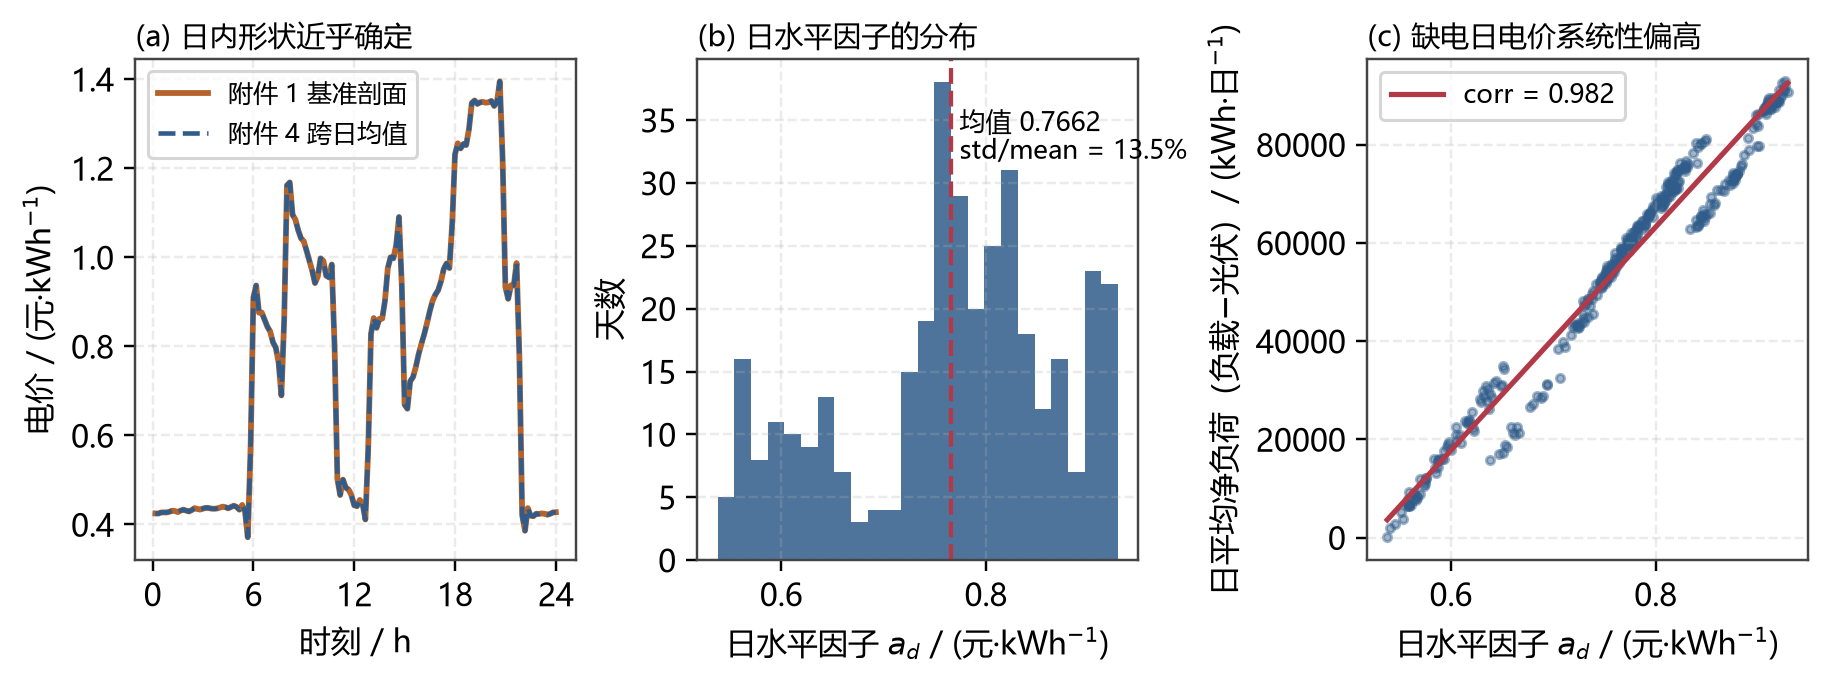
\includegraphics[width=0.99\textwidth]{figures/fig_q4_price.png}
  \caption{附件 4 的电价结构：日内形状、日水平分布与缺电日相关性}
  \label{fig:q4price}
\end{figure}

\noindent 图 \ref{fig:q4price} 的三个面板与上述三项统计一一对应。
\emph{(a)} 把附件 4 每天的电价减去\emph{当天均值}得到该日的“形状”，再对 334 天求
平均，与附件 1 的基准剖面画在一起：两条线几乎完全重合，说明附件 4 的日内形状就是
附件 1 的典型日分时剖面，逐日变化几乎只体现为整体平移——这就是“日内形状占总方差
$84.6\%$”的直观形式。\emph{(b)} 日水平因子 $a_d$（当天 144 槽电价的平均）的直方图，
均值 0.7662 元/kWh、$std/mean=13.5\%$，即逐日浮动的是“整天买电贵不贵”，而不是
“哪个时段贵”。\emph{(c)} 日水平因子对日均净负荷（当日负载减光伏）的散点，一个点
代表一天，线性拟合的相关系数为 0.982：\emph{缺电日的电价系统性偏高}。
三个面板合起来给出 §\ref{sec:q4model} 建模的关键前提——价格逐日只在“整体水平”上
浮动（b），而这一浮动是对全天的\emph{均匀平移}、不改变日内形状（a）。

\noindent（2）分析得到的结论。式 \eqref{eq:q3cost} 的四项收费
$p\hat g$、$0.5p$、$1.5p$、$5p$ 都是同一个 $p$ 的倍数，而日水平因子是\emph{全天
均匀平移}；均匀平移不改变任何边际权衡。因此价格的整体水平只按比例影响账单、
不影响最优决策，能够影响决策的只有日内残差部分（占总方差 $6.2\%$）。

\noindent（3）据此确定的模型改动范围。问题四不改变储能物理、决策变量的
边界、可交付结构与结算口径，只改变价格的进入方式：计划层的价格系数取公布的分时
电价剖面，称部分信息口径，即 0:00 只知道公布的分时电价、不知道当天
实际电价；或取当天实际电价，称完全信息口径，用作价格信息的下界。
结算与写盘一律使用附件 4 的实际价。问题四-二还需把紧急购电的场景系数由标量
$5p$ 改为逐场景逐槽 $5p_{\omega,t}/K$，使价格与缺口的联合分布进入决策。

\subsection{数据预处理与建模口径}

\noindent（1）附件 1 是全年平均典型日。附件 1 的电价、负载、光伏分别等于
附件 4 与附件 2 的全年平均，光伏因四位小数舍入相差 0.04 kW，故问题一的确定性求解
可直接以附件 1 为输入。

\noindent（2）时间标签取右端点解读。附件 1/2/4 的时间列取右端点语义，
即 $0{:}10$ 代表区间 $[0{:}00,0{:}10]$，144 个区间恰好覆盖全天。附件 5 的模板行
标签是起止点标注且自 $0{:}10$-$0{:}20$ 起步，故写入结果文件时按
$\text{result}[k]=p[(k+1)\bmod 144]$ 作标签对齐。

\noindent（3）附件 3 只给出\emph{整点时刻}的光伏预报，而解算需要 10 分钟粒度的逐槽
输入。若按分段常数把整点值摊平到其后六个槽，正午单峰会被削成台阶、预报系统性偏低，
计划层随之过度购电。该预报的物理含义是这一整点\emph{时刻}取值的含噪副本，而非小时
平均功率，本文据此把它\textbf{线性插值}到 10 分钟粒度使用。附件 3 本身近乎无偏
（全年总量误差约 $1.2\%$），误差随预报时距近似减半（0:00 档报正午的 RMSE 约
766 kW、6:00 档约 471 kW），按原义使用才能保住这份精度：实测正午净需求的预报误差
由分段常数的 \textbf{867 kW} 降至 \textbf{524 kW}。逐档、逐时窗的 RMSE 对比见
\S\ref{sec:q3result} 的图 \ref{fig:q3rmse}。

\noindent（4）负荷没有预报，须自行构造基线。本文按暖机期的日均净负荷把
七天分为低需求日与其余两组，以回看窗口内同组历史日的均值作为负荷基线，其构造
详见 \S\ref{sec:q2scen}；问题三采用同一构造，仅回看窗口略有不同。

\begin{figure}[!htbp]
  \centering
  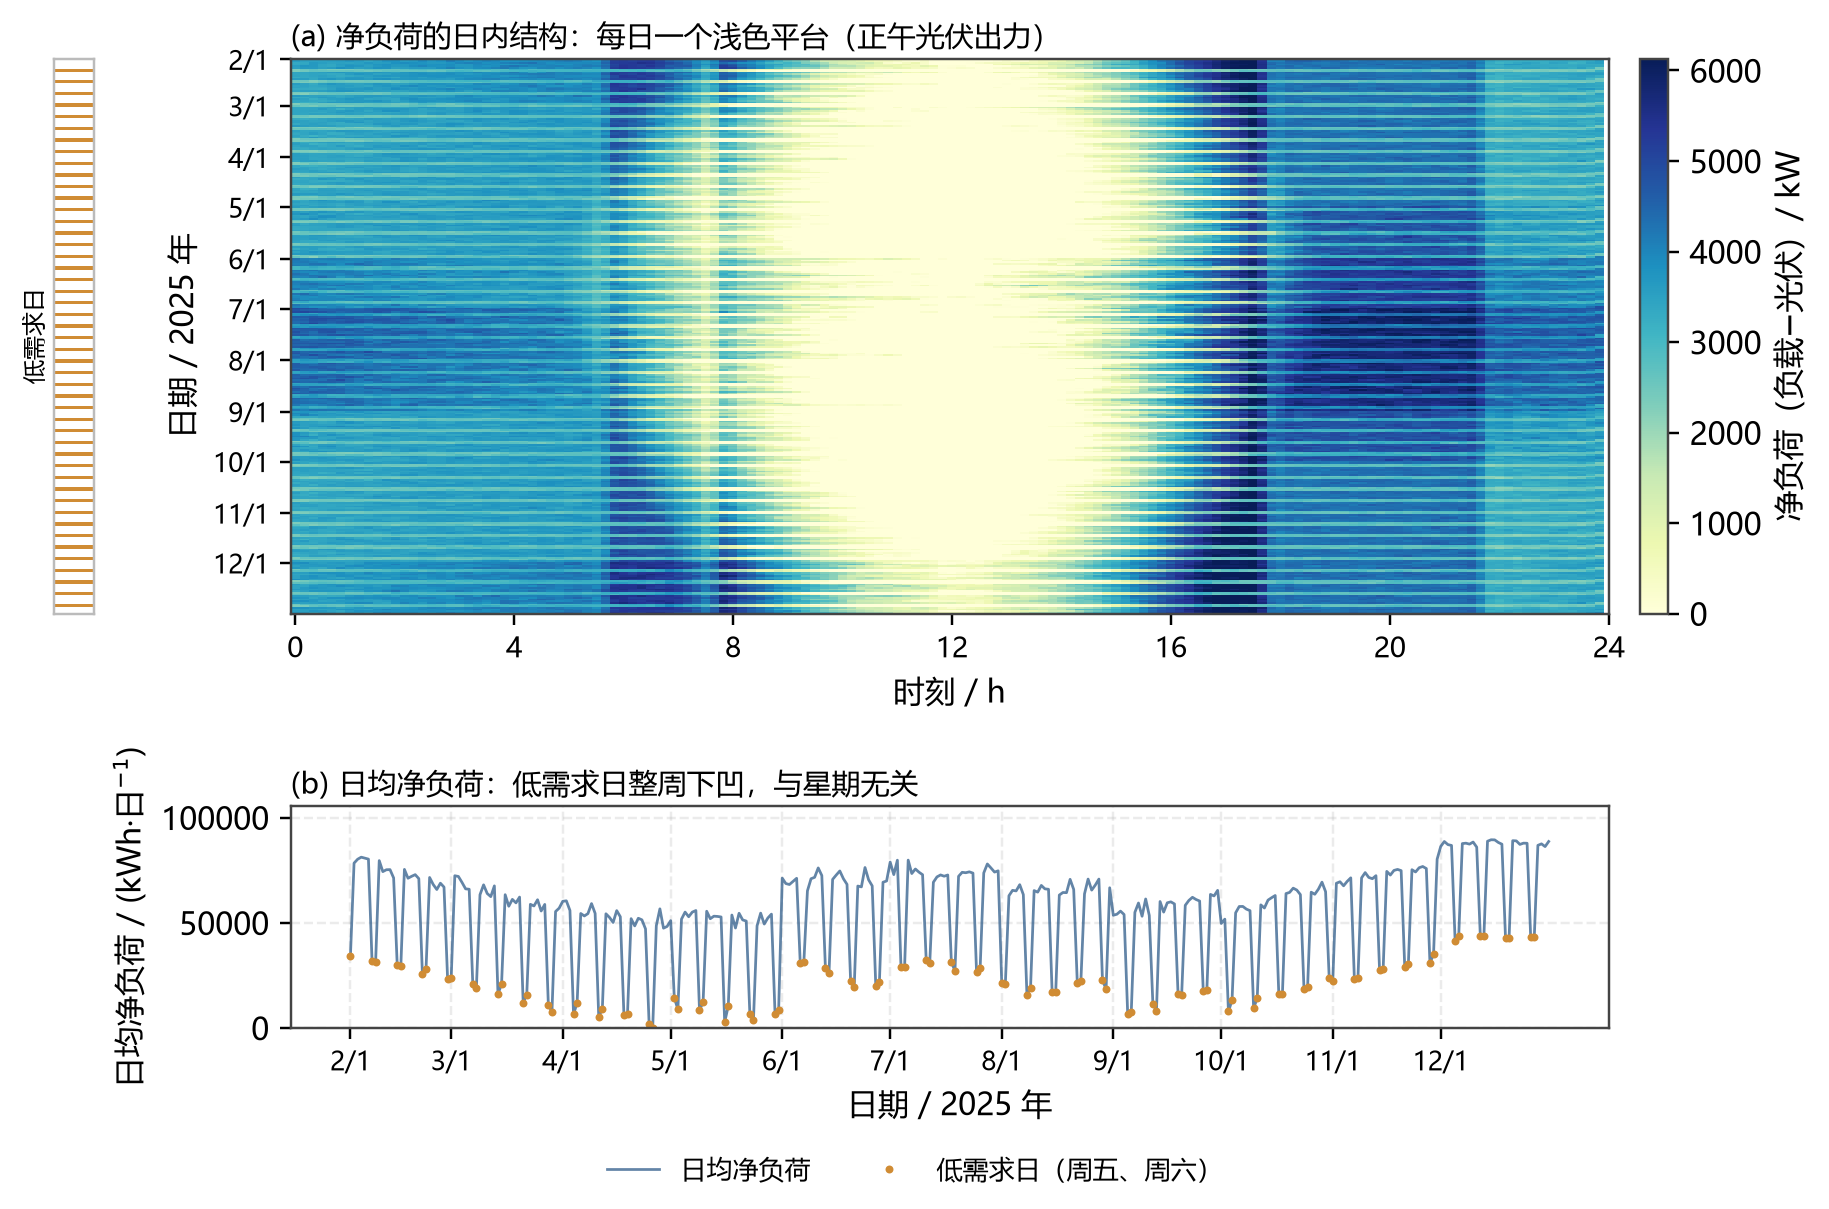
\includegraphics[width=0.95\textwidth]{figures/fig_q2_netheat.png}
  \caption{全年净负荷的日内结构与逐日水平（计费窗口 334 天；左侧细带为由暖机期
  推出的低需求日标记）}
  \label{fig:q2netheat}
\end{figure}

\noindent 图 \ref{fig:q2netheat} 给出该规则的数据依据。(a) 的日内结构显示，每天
正午都出现一个浅色平台（光伏出力最大），逐日差别只体现在整行水平上；(b) 的日均
净负荷整年呈严格周周期，每周固定两天跌到其余五天的约三分之一，且这两天是周五与
周六，而周日与周一至周四齐平、并不低。可见：（1）区分各日的不是星期而是用电水平，
按日历直觉把周末当作低需求日是错的；（2）这一差距在整年上稳定存在，故只用暖机期
（前 31 天）推出的规则可以套用到整个计费窗口。

\noindent（5）统计窗口。问题 2、3、4 统一取 2025 年 2 月 1 日至 12 月 31 日
共 334 天，1 月作为暖机期。

% ===================================================================== §3
\section{模型假设}
\label{sec:assume}

为简化模型并保证可解性，本文作出如下假设：

\noindent \textbf{假设 1}（效率口径）：储能设备标注的 90\% 效率指充电与放电\emph{各}
打 9 折，即往返效率为 $0.9\times0.9=81\%$。\\
\emph{依据}：附录 1 只给出单一效率数值而未区分方向。该口径是较保守的一种解读；
作为对照，若按往返效率 90\%（每程 $\sqrt{0.9}$）理解，问题 1 的结果为
57\,526.24 kWh / 33\,801.50 元，与本文口径相差 $3.8\%$，该差异已在
\S\ref{sec:q1result} 中报告。

\noindent \textbf{假设 2}（不向电网售电）：微网只能向外部电网购电，不能售电；光伏
发电量超过负载与储能可吸收部分时作弃光处理。\\
\emph{依据}：题面只给出购电价而未给售电价，附件 5 的输出表也只要求填写购电量。

\noindent \textbf{假设 3}（紧急购电的触发口径）：紧急购电的触发条件是\emph{微网供电
低于小区负载}，即 $e_t=\max(0,\,L_t-g_t-P_t-d_t)$，不把计划充电量计入必须执行的量。\\
\emph{依据}：问题 2 原文为“如果低于负载，需向外网紧急购电”，触发条件明确指向
负载缺口而非“计划未完成量”。

\noindent \textbf{假设 4}（时间标签）：附件 1/2/4 的时间标签为右端点标注，$0{:}10$
表示区间 $[0{:}00,0{:}10]$。\\
\emph{依据}：只有右端点解读才能使日期在 $00{:}00$--$24{:}00$ 内完整排布。

\noindent \textbf{假设 5}（预报的物理含义）：附件 3 中“预报 $k$ 小时”给出的是发布
时刻之后第 $k$ 个小时整点\emph{时刻}功率的预报值，使用前线性插值到 10 分钟。\\
\emph{依据}：对附件 3 与实际光伏的配对检验表明它是单点值的含噪副本，而非小时平均
功率。

\noindent \textbf{假设 6}（购电功率的读法，非自加假设）：问题 2、3 均\emph{不}对购电
功率设上界，即按题面字面读法取 $G\ge0$。\\
\emph{依据}：题面（附录 1）只给出了储能的最大充放电功率 5000 kW，并未给出
微网与外网的联络线容量，故上界本身不由题面给出、属于\emph{读法选择}。本文主交付取
字面读法（不设上界）；作为对照，\S\ref{sec:sens} 同时给出 $G\le5000$ kW 保守读法
下的可交付结果，并说明两套数值不可混排。

\noindent \textbf{假设 7}（终端电量，自加假设）：问题 2、3、4 附加全年能量中性约束
$SOC_0=SOC_T=6000$ kWh。\\
\emph{依据}：题面仅在问题 1 中要求首末储电量相等，问题 2--4 未作要求。若不施加该
约束，最优解会把一池电量留在电池中收尾（相当于无偿多得），使跨年比较失去意义，
故本文统一按问题 1 的口径处理，并在结果中说明实际执行层的末值。

\noindent \textbf{假设 8}（忽略电池退化成本）：不计入储能设备的循环寿命损耗成本。\\
\emph{依据}：题面未给出任何退化参数。这是本文相对部分既有微网调度研究的\emph{主动
偏离}，会使模型倾向于更充分地使用电池，故在 \S\ref{sec:eval} 的模型局限中一并说明。

% ===================================================================== §4
\section{符号说明}

{\zihao{-5}
\begin{longtable}{c l c c}
  \caption{符号说明}\label{tab:notation}\\
  \toprule[1.5pt]
  \hd{符号} & \hd{含义} & \hd{单位} & \hd{类型}\\
  \midrule[1pt]
  \endfirsthead
  \multicolumn{4}{l}{\zihao{-5} 续表：符号说明}\\
  \toprule[1.5pt]
  \hd{符号} & \hd{含义} & \hd{单位} & \hd{类型}\\
  \midrule[1pt]
  \endhead
  \endlastfoot
    $t$              & 时间区间序号，$t=0,1,\dots,143$              & ---   & 下标\\
    $\Delta t$       & 单个时间区间长度，$1/6$                       & h     & 常量\\
    $p_t$            & 外网电价（附件 1 基准剖面）                    & 元/kWh & 参数\\
    $p_{d,t}$        & 第 $d$ 天第 $t$ 槽的实际结算电价（附件 4）      & 元/kWh & 参数\\
    $L_t$            & 小区负载功率（附件 2）                         & kW    & 参数\\
    $P_t$            & 光伏发电实际功率（附件 2）                      & kW    & 参数\\
    $\hat P_t$       & 光伏发电预报功率（附件 3）                      & kW    & 参数\\
    $F_t$            & 净需求（负荷减光伏），$F_t=L_t-P_t$             & kW    & 参数\\
    \midrule[1pt]
    $g_t$            & 购电功率                                     & kW    & 决策变量\\
    $\hat g_t$       & 计划购电功率（0:00 制定）                      & kW    & 决策变量\\
    $c_t,\ d_t$      & 储能充电、放电功率                             & kW    & 决策变量\\
    $s_t$            & 弃光功率                                     & kW    & 决策变量\\
    $e_t$            & 紧急购电功率                                  & kW    & 决策变量\\
    $SOC_t$          & 第 $t$ 区间起始时刻的储电量                     & kWh   & 状态变量\\
    \midrule[1pt]
    $P_{\max}$       & 储能最大充放电功率，5000                       & kW    & 常量\\
    $G_{\max}$       & 购电功率上界（读法约定，见假设 6；保守读法取 5000）      & kW    & 常量\\
    $SOC^{\min},SOC^{\max}$ & 储电量下限、上限，1200 / 10800          & kWh   & 常量\\
    $\eta$           & 单程充放电效率，0.9                            & ---   & 常量\\
    \midrule[1pt]
    $\gamma$         & 覆盖率的可交付水平（\S\ref{sec:q2model}）      & ---   & 参数\\
    $q_{\gamma,t}$   & 区间 $t$ 的可交付充电下确界                     & kW    & 参数\\
    $\tau,\ \tau'$   & 盲窗（第 0 块）、可调段（后三块）的对冲分位      & ---   & 参数\\
    $r$              & 水平校正比值（已发生时段实测负荷与基准之比）     & ---   & 参数\\
    $\Omega$         & 低需求日分组的历史日构成的情景集                 & ---   & 集合\\
    $Z$              & 全天（或全窗口）总购电费                        & 元    & 目标\\
    \bottomrule[1.5pt]
\end{longtable}
}

% ===================================================================== §5
\section{模型的建立与求解}

\subsection{问题一：确定性线性规划购电模型}
\label{sec:q1model}

\subsubsection{模型建立}

将一天离散为 $144$ 个长度为 $\Delta t=1/6$ h 的区间，$t=0,1,\dots,143$。
每个区间的决策变量为：购电功率 $g_t$、充电功率 $c_t$、放电功率 $d_t$ 与弃光功率 $s_t$；
状态变量为区间起始时刻的储电量 $SOC_t$。以全天购电费最小为目标，
确定性线性规划模型如下所示：

\begin{equation}
\begin{gathered}
\min_{g,c,d,s,SOC}\; Z_1=\sum_{t=0}^{143} p_t\,g_t\,\Delta t\\[2pt]
\text{s.t.}\;
\begin{cases}
g_t+P_t+d_t=L_t+c_t+s_t, & \text{（功率平衡）}\\
SOC_{t+1}=SOC_t+\eta\,c_t\Delta t-\dfrac{d_t\Delta t}{\eta}, & \text{（储电递推）}\\
SOC^{\min}\le SOC_t\le SOC^{\max},\; SOC_0=SOC_{144}=6000,
  & \text{（电量区间与首末相等）}\\
0\le c_t\le P_{\max},\; 0\le d_t\le P_{\max},\; g_t,s_t\ge0,
  & \text{（功率上限与非负）}
\end{cases}
\end{gathered}
\label{eq:q1model}
\end{equation}

上式即本文所称的基于储能峰谷套利的单日确定性线性规划购电模型，
共含 $144\times4+145=721$ 个决策变量与 $288$ 条等式约束。模型无需再添加
$c_td_t=0$ 这类互补约束：同一区间若同时充放电，净电量变化为
$\eta-1/\eta=-0.19<0$，纯属亏能量，最优解中不会出现。弃光量也不必额外惩罚：
光伏发电不产生费用而购电需要付费，优化器会自动优先消纳光伏。

\subsubsection{模型求解}

模型为纯线性规划：读入附件 1 的 144 个 10 分钟区间数据后，按式 \eqref{eq:q1model}
组装系数矩阵（共 721 个决策变量、288 条等式约束），以
\texttt{scipy.optimize.linprog} 接口调用 HiGHS 求解器（\texttt{method=“highs”}）
求解，最后检验功率平衡残差、储电量边界与首末值并输出结果。求解器返回状态
\texttt{Optimal}，耗时在毫秒量级。求解流程如图 \ref{fig:q1flow} 所示。

\begin{figure}[!htbp]
  \centering
  \begin{tikzpicture}[node distance=6.5mm and 8mm]
    \node[databox] (a) {读取附件 1\\144 区间电价/负载/光伏};
    \node[box, right=of a] (b) {离散化\\$\Delta t=1/6$ h，$t=0..143$};
    \node[box, right=of b] (c) {构造 LP\\721 变量 / 288 等式};
    \node[box, below=of c] (d) {调用 HiGHS\\求得全局最优解};
    \node[box, left=of d] (e) {约束自检\\功率平衡残差/SOC 边界};
    \node[resbox, left=of e] (f) {输出 result1.xlsx\\表 2、表 3};
    \draw[ar] (a) -- (b);  \draw[ar] (b) -- (c);  \draw[ar] (c) -- (d);
    \draw[ar] (d) -- (e);  \draw[ar] (e) -- (f);
  \end{tikzpicture}
  \caption{问题一的求解流程}
  \label{fig:q1flow}
\end{figure}

\subsubsection{求解结果}
\label{sec:q1result}

\begin{table}[!htbp]
  \centering
  \caption{问题一：微网在指定时间段的购电量及全天的购电量和购电费}
  \label{tab:q1t1}
  \zihao{-5}
  \begin{tabular}{c c c c c c}
    \toprule[1.5pt]
    \hd{时间段} & \hd{购电量/kWh} & \hd{时间段} & \hd{购电量/kWh} & \hd{时间段} & \hd{购电量/kWh}\\
    \midrule[1pt]
    10:00-10:10 & 0.00 & 12:00-12:10 & 480.41 & 14:00-14:10 & 0.00\\
    16:00-16:10 & 445.43 & 18:00-18:10 & 531.89 & 20:00-20:10 & 0.00\\
    \midrule[1pt]
    \multicolumn{2}{c}{\hd{全天购电量：59\,482.70 kWh}}
      & \multicolumn{4}{c}{\hd{全天购电费：35\,126.95 元}}\\
    \bottomrule[1.5pt]
  \end{tabular}
\end{table}

\begin{table}[!htbp]
  \centering
  \caption{问题一：储能设备在指定时间段的充放电量及 0:00 和 24:00 的储电量}
  \label{tab:q1t2}
  \zihao{-5}
  \begin{tabular}{c c c c c c}
    \toprule[1.5pt]
    \hd{时间段} & \hd{充电量/kWh} & \hd{放电量/kWh} & \hd{时间段} & \hd{充电量/kWh} & \hd{放电量/kWh}\\
    \midrule[1pt]
    0:00-4:00   & 4500.00 & 0.00     & 4:00-8:00   & 833.33  & 6365.84\\
    8:00-12:00  & 4787.96 & 1703.00  & 12:00-16:00 & 5286.04 & 91.10\\
    16:00-20:00 & 0.00    & 5780.13  & 20:00-24:00 & 5333.33 & 2859.87\\
    \midrule[1pt]
    \multicolumn{2}{c}{\hd{0:00 储电量：6000.00 kWh}}
      & \multicolumn{3}{c}{\hd{24:00 储电量：6000.00 kWh}}\\
    \bottomrule[1.5pt]
  \end{tabular}
\end{table}

\subsubsection{结果分析与检验}

图 \ref{fig:q1day} 给出全天电价、负载、光伏与计划购电量的对照。表 \ref{tab:q1t2}
只列出 6 个 4 小时块的充放电聚合量与两个储电量锚点，看不出充放电发生在什么时刻，
故图 \ref{fig:q1soc} 进一步给出储电量的时序轨迹与电价背景的对应关系。

\begin{figure}[!htbp]
  \centering
  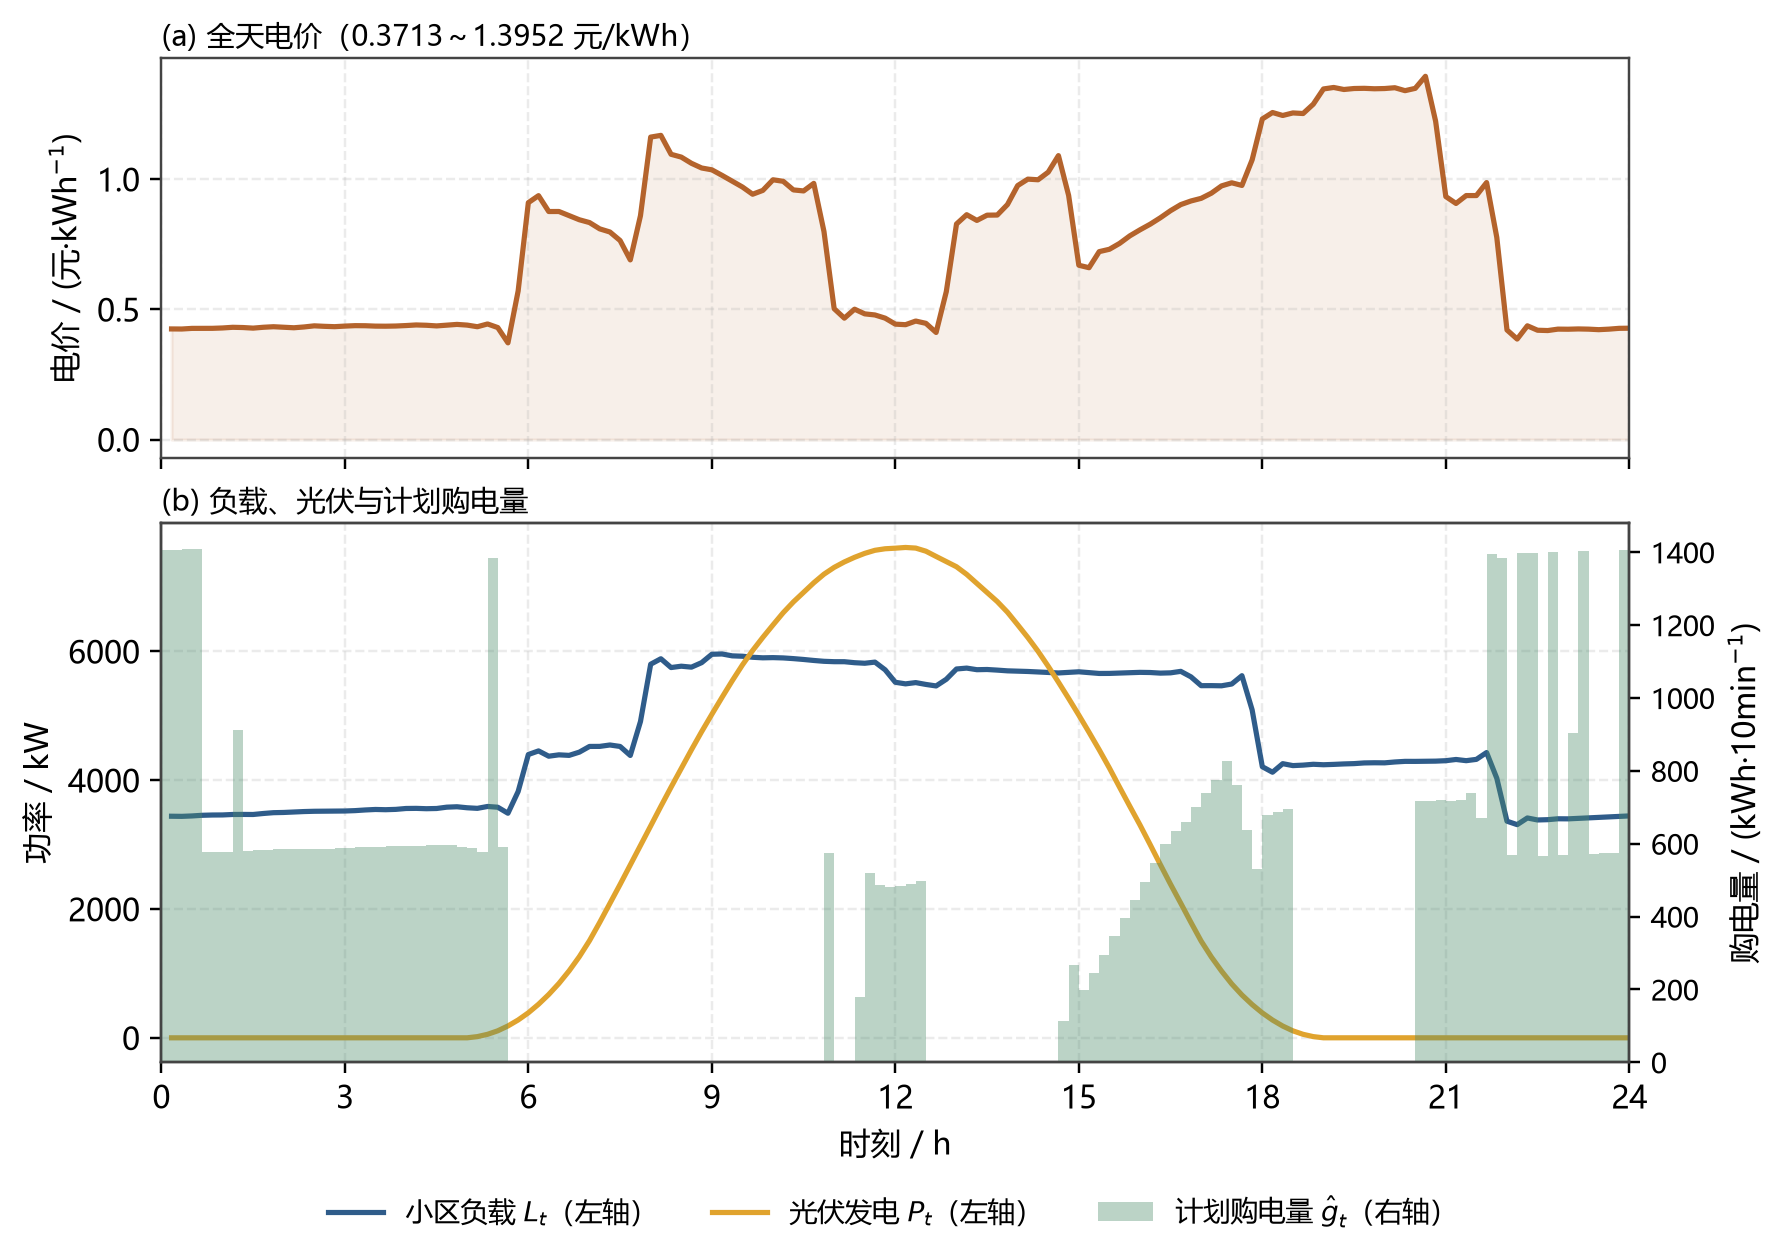
\includegraphics[width=0.80\textwidth]{figures/fig_q1_day.png}
  \caption{问题一：全天电价、负载、光伏与计划购电量}
  \label{fig:q1day}
\end{figure}

\begin{figure}[!htbp]
  \centering
  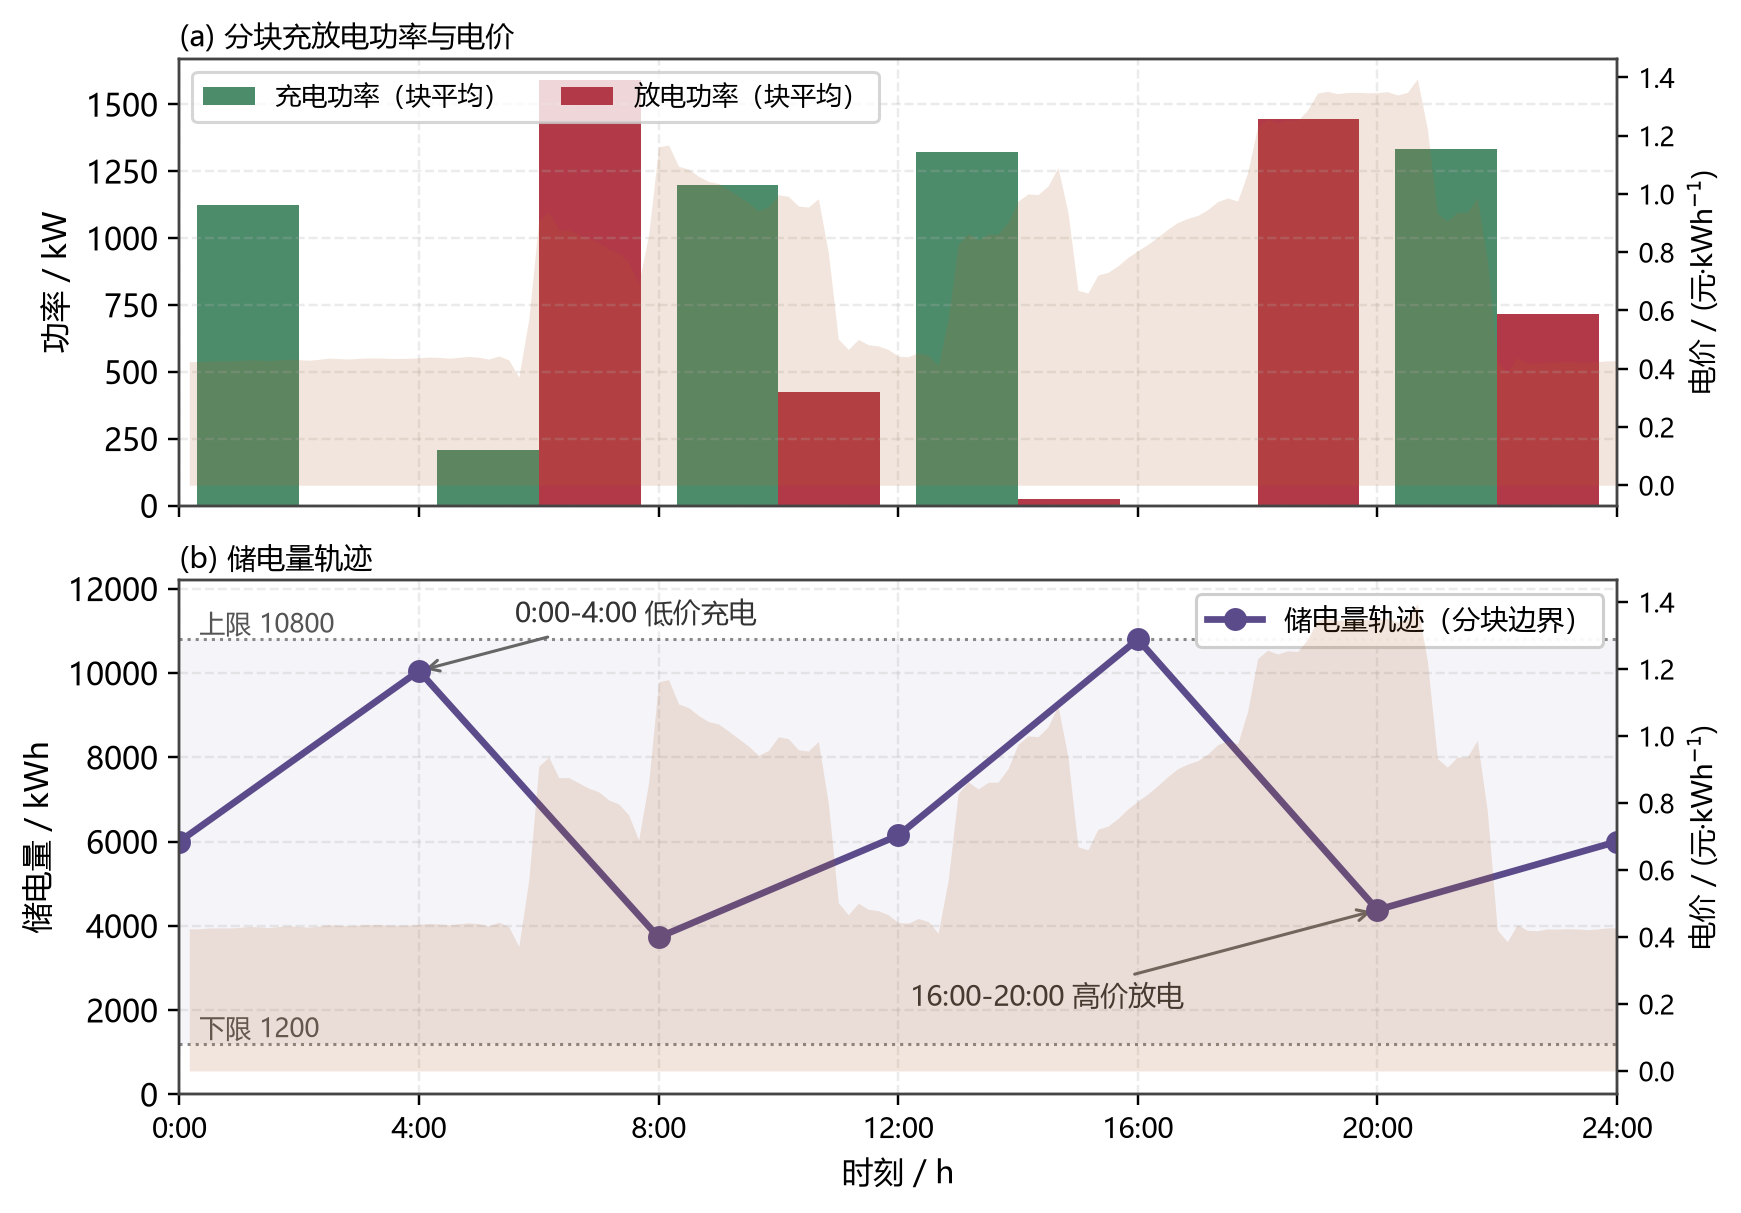
\includegraphics[width=0.82\textwidth]{figures/fig_q1_soc.png}
  \caption{问题一：分块充放电功率与储电量轨迹}
  \label{fig:q1soc}
\end{figure}

由上述结果可以得出以下结论：

\begin{enumerate}[itemsep=1pt, topsep=2pt]
  \item 储能套利是费用下降的唯一来源。凌晨电价最低（约 0.42 元/kWh）的
        0:00--4:00 区间充电 4500.00 kWh；早高峰（4:00--8:00，电价升至约 0.9--
        1.16 元/kWh）与晚高峰（16:00--20:00，电价约 1.2--1.4 元/kWh）分别放电
        6365.84 kWh 与 5780.13 kWh。购电量被系统性地从高价时段转移到低价时段。
  \item 光伏实现零弃光。全天光伏总能量 55\,483 kWh 恰好可被负载与储能
        全部吸收，弃光量为 0。
  \item 电池被充分利用。储电量在一天内触及上下限两侧边界，全天充电
        20\,740.67 kWh，约为可用容量区间（9600 kWh）的 2.16 倍，即完成约两次
        满充满放循环。
  \item 效率损耗是可量化的套利成本。全天购电量 59\,482.70 kWh 与净负荷
        55\,541.97 kWh 之差为 3940.73 kWh，恰等于充电量的 $19\%$，即往返效率
        81\% 所导致的能量损失。
\end{enumerate}

\noindent 模型检验。对上述解作六项自检，全部通过：求解状态为
\texttt{Optimal}（HiGHS），即全局最优；功率平衡的最大残差为
$1.82\times10^{-12}$ kW；储电量取值范围为 $[1200.0000,\ 10800.0000]$ kWh，
既落在安全区间内又触及两端边界（满利用）；储电量首末值均为 6000.0000 kWh；
放电量与充电量之比为 $0.81$，与往返效率一致；弃光量为 0 kWh，光伏被全部消纳。

\noindent 效率口径的敏感性。按假设 1 的对照口径（往返效率 90\%，即每程
$\sqrt{0.9}$）重解，全天购电量降为 57\,526.24 kWh、购电费降为 33\,801.50 元，
与本文口径相差 $3.8\%$。该差异不改变最优策略的结构（仍是“夜间充电、峰时放电”），
只改变套利的经济幅度。

\subsection{问题二：$\gamma$-可交付储能计划的两阶段购电优化模型}
\label{sec:q2model}

\subsubsection{建模口径与决策变量的边界}

题面要求“每天 0:00 制定当天的计划购电策略”，因此 0:00 能够承诺的量只有计划购电量
$\hat g_t$；储能充放电 $c_t,d_t$ 与紧急购电 $e_t$ 都由当天实际发生的负载与光伏决定，
是实时追索量。本文据此把模型分为规划层与执行层两层，并令两层共用同一套储能
物理：规划层的储电递推以“可得充电量下确界”为依据（见下文），执行层则严格按实际
发生的负载与光伏推进储电量。这样组织的模型能保证规划层承诺的放电量在任何情景下都
物理可得，报出的总费用也不会低于“同一计划下储能完美预见”的理论下界。

\subsubsection{模型建立}

\noindent（1）可交付充电下确界。为使规划层的储能递推在\emph{所有}情景下都
可执行，本文用“可得充电量下确界”替换递推式中的期望充电量。设情景集 $\Omega$ 由
历史日构成，其构造方式见下节；定义覆盖率 $\gamma$ 下的可交付充电下确界为净富余
$q_{\gamma,t}$，其计算公式如下所示：

\begin{equation}
c_t^{\min}\;\le\;\hat g_t+d_t+q_{\gamma,t},
\qquad
q_{\gamma,t}=\bigl\{\,P_{\omega,t}-L_{\omega,t}\,\bigr\}_{\omega\in\Omega}
\text{ 的 }(1-\gamma)\text{ 分位数}.
\label{eq:q2gamma}
\end{equation}

在上式中，$c_t^{\min}$ 为区间 $t$ 的可得充电量下确界，$\Omega$ 为历史日构成的情景集。
$\gamma=1$ 时 $q_t=\min_{\omega}(P_{\omega,t}-L_{\omega,t})$，即逐情景
全部可交付，此时规划层与执行层的储能物理完全一致，不存在模拟歧义；且目标
函数中的 $e$ 只依赖 $(\hat g,d)$ 而与储电量无关，因此给定 $(\hat g,d)$ 的总费用是
\emph{闭式}的，不需要任何执行层模拟。

\noindent（2）规划层。以计划购电费最小为目标，同时计入情景平均紧急购电费，
规划模型如下所示：

\begin{equation}
\begin{gathered}
\min_{\hat g,\hat c,\hat d,\hat s,SOC}\; Z_2=\sum_{t}p_t\hat g_t\Delta t
      +\mathbb{E}_{\omega}\!\left[\sum_t 5p_t e_{\omega,t}\Delta t\right]\\[2pt]
\text{s.t.}\;
\begin{cases}
\hat g_t+\hat P_t+\hat d_t=\hat L_t+\hat c_t+\hat s_t, & \text{（功率平衡）}\\
SOC_{t+1}=SOC_t+\eta\,c_t^{\min}\Delta t-\dfrac{\hat d_t\Delta t}{\eta}, & \text{（可交付储电递推）}\\
SOC^{\min}\le SOC_t\le SOC^{\max},\; SOC_0=SOC_{T}=6000,
  & \text{（电量区间与全年中性）}\\
0\le \hat c_t,\hat d_t\le P_{\max},\; \hat g_t\ge0,\; \hat s_t\ge0,
  & \text{（功率上限与非负）}
\end{cases}\\[2pt]
c_t^{\min}\ \text{由式}\eqref{eq:q2gamma}\ \text{给出},\; t=0,1,\dots,T-1
\end{gathered}
\label{eq:q2model}
\end{equation}

\noindent 式中 $T=365\times144=52\,560$ 为全年槽数（1 月为暖机期，计费窗口取
2/1--12/31 的 334 天，即 48\,096 槽），即计划\emph{一次}联立求解整年（情景集按日
取自同组历史日），购电功率不设上界。与逐日独立求解相比，全年联立只多出“年末回归”
这一层耦合，实测两者相差 14\,766 元（$0.108\%$，见 \S2.3 之(3)），故下文按日解释
执行层不失一般性。

\noindent（3）执行层（严格储电量因果策略）。执行层不使用任何跨时段的值
函数近似，而按“当前缺口优先”的因果规则逐槽推进，具体步骤如下：

\begin{enumerate}[label=Step \arabic*., leftmargin=*, itemsep=2pt, topsep=3pt]
  \item 计算当前缺口并放电。
        \[
        \Delta_t^{-}=\max\bigl(0,\ L_t-P_t-\hat g_t\bigr),\qquad
        d_t=\min\Bigl(\Delta_t^{-},\ P_{\max},\
                 \frac{(SOC_t-SOC^{\min})\,\eta}{\Delta t}\Bigr);
        \]
  \item 计算富余电量并充电。
        \[
        \Delta_t^{+}=\max\bigl(0,\ P_t+\hat g_t+d_t-L_t\bigr),\qquad
        c_t=\min\Bigl(\Delta_t^{+},\ P_{\max},\
                 \frac{SOC^{\max}-SOC_t}{\eta\,\Delta t}\Bigr);
        \]
  \item 结算紧急购电。
        \[
        e_t=\max\bigl(0,\ L_t-P_t-\hat g_t-d_t\bigr);
        \]
  \item 更新储电量。按储能递推式
        $SOC_{t+1}=SOC_t+\eta c_t\Delta t-d_t\Delta t/\eta$ 推进至下一区间。
\end{enumerate}

该策略只使用当前时刻的实际负载、光伏与储电量，逐槽严格满足储电量递推与上下限
约束，因此是可执行的。

\noindent（4）完美预见下界（哨兵）。为检验模型是否被放松，本文另计算
“同一计划下储能完美预见”的理论下界，作为所有结果的哨兵：任何低于该下界的结果
都必然是模型错误。

\noindent 模型命名：本文将式 \eqref{eq:q2gamma}--\eqref{eq:q2model} 连同
哨兵检验合称为基于可交付储能计划与严格储电量因果执行的两阶段购电优化模型。

\subsubsection{情景集的构造：低需求日分组}
\label{sec:q2scen}

可交付下确界 $q_{\gamma,t}$ 的取值由情景集 $\Omega$ 决定，而它又决定了计划量的对冲
水位。情景集怎么构造，计划层的对冲水位就怎么定，这是问题二中最关键的一步建模决策。

本文的构造依据来自附件 2 中一个容易被忽略的事实：真正区分各日的并不是星期，而是
\emph{用电水平}（见图 \ref{fig:q2netheat}）。周五与周六的日均净负荷分别为
22\,481 与 22\,887 kWh，其余五天均在 6.8 万 kWh 上下，两者相差近三倍；周日则不然，
其日均净负荷为 68\,386 kWh，与周一至周四基本持平，呈现典型的工作日特征。

据此，本文以\emph{暖机期}（前 31 天，位于计费窗口之前）的日均净负荷为准则，把七天
划分为低需求日与其余日两组，再取回看 6 天内与当日同组的历史日作为情景集。分组规则
只喂暖机期，在计费窗口开始前即已固定，故不存在前视。以 1--6 月、全年或报告窗口
分别推导，得到的低需求日都是周五与周六，说明该划分对推导窗口并不敏感。

表 \ref{tab:q2scen} 在 $\gamma=1$ 可交付计划下比较了各种构造。

\begin{table}[!htbp]
  \centering
  \caption{两种情景集构造的结果对比（$\gamma=1$，窗口 2/1--12/31）}
  \label{tab:q2scen}
  \zihao{-5}
  \begin{tabular}{l r r r}
    \toprule[1.5pt]
    \hd{分组方式与回看窗口} & \hd{平均情景数} & \hd{实际执行总费/元} & \hd{判定}\\
    \midrule[1pt]
    同星期几 $K=4$（对照）        & 3.81 & 15\,134\,192 & 基线\\
    同星期几 $K=2$                & 1.94 & 15\,041\,540 & 不显著\\
    低需求日分组，回看 6 天（定稿） & 3.12 & 13\,846\,553
      & 显著\\
    \quad 分组，回看 14 天        & 8.11 & 14\,341\,723 & 显著\\
    \quad 日历周末 $\{$周六, 周日$\}$，回看 6 天 & 3.12 & 22\,104\,625
      & 显著更差\\
    \quad 不分组（全七天），回看 6 天 & 5.94 & 16\,403\,378 & 显著更差\\
    \midrule[1pt]
    定稿相对基线节省 & & $1\,287\,639$（$8.51\%$） & \\
    \bottomrule[1.5pt]
  \end{tabular}

  \vspace{2pt}
  \parbox{0.95\textwidth}{\zihao{-5} 注：「实际执行总费」由执行层按实际缺口重算
  放电后结算，即表 \ref{tab:q2summary} 的交付值。回看窗口小于 6 天时，低需求日
  每周只有两天，窗口内取不到同组历史日，程序会退回用当日自身充当情景天而形成前视，
  故不采用。}
\end{table}

对照组的同星期几构造总费为 1\,513.42 万元，低需求日分组将其降至
1\,384.66 万元，节省 128.76 万元，降幅达 $8.51\%$。这一降幅超过本文在
问题二上任何一项算法改动的效果。

分组方式必须由数据推出，不能按日历直觉设定。改按日历周末（周六、周日）取样，
总费升至 2\,210.46 万元，比对照组高 697.04 万元；完全不分组，亦高出 126.92 万元。
原因即前文所述：数据中的周日是工作日，将其与周六并入同一情景集，等于混淆了两种
用电水平。

回看窗口取 6 天有其必然性。低需求日每周仅两天，窗口取 6 天才能使周五与周六各得
1 个同组历史日；窗口缩至 5 天，窗内已无同组历史日，程序将退回以当日自身充当情景天，
形成前视，故不予采用。窗口延长至 14 天以上则引入季节漂移，总费回升至 1\,434.17
万元，21 天为 1\,471.35 万元。

\subsubsection{模型求解}

求解过程为：先由附件 2 按低需求日分组得到情景集 $\Omega$，按式
\eqref{eq:q2gamma} 逐区间计算可交付下确界 $q_{\gamma,t}$ 并取 $\gamma=1$；
再求解式 \eqref{eq:q2model} 得到计划购电量 $\hat g$ 与计划充放电量；最后在 2025 年
实际轨迹上执行 \S5.2.2 之(3) 的因果策略，重算充放电量、紧急购电量、费用与储电量
轨迹并写入结果文件。流程如图 \ref{fig:q2flow} 所示。

\begin{figure}[!htbp]
  \centering
  \begin{tikzpicture}[node distance=6.5mm and 6.5mm]
    \node[databox] (a) {附件 2\\全年负载/光伏};
    \node[box, right=of a] (b) {构造低需求日\\分组情景集 $\Omega$};
    \node[box, right=of b] (c) {计算可交付\\充电下确界 $q_{\gamma,t}$};
    \node[box, below=of c] (d) {求解 $\gamma=1$\\规划 LP};
    \node[box, left=of d] (e) {因果执行层\\按缺口优先逐槽推进};
    \node[warnbox, left=of e] (g) {哨兵检验\\$\ge$ 完美预见下界};
    \node[resbox, below=of e] (f) {输出 result2.xlsx};
    \draw[ar] (a) -- (b); \draw[ar] (b) -- (c); \draw[ar] (c) -- (d);
    \draw[ar] (d) -- (e); \draw[ar] (e) -- (g); \draw[ar] (e) -- (f);
  \end{tikzpicture}
  \caption{问题二的求解流程}
  \label{fig:q2flow}
\end{figure}

\subsubsection{求解结果}

\noindent（1）覆盖率的选取。$\gamma$ 是规划层的唯一自由度，表
\ref{tab:q2gamma} 给出一维扫描结果。$\gamma<1$ 的各档虽然名义费用更低，但计划层
不可交付（情景中会违反储电量约束），只有 $\gamma=1$ 一行可以作为规划输入。

\begin{table}[!htbp]
  \centering
  \caption{规划层覆盖率 $\gamma$ 的敏感性（窗口 2/1--12/31，共 334 天）}
  \label{tab:q2gamma}
  \zihao{-5}
  \begin{tabular}{c r r r r c}
    \toprule[1.5pt]
    \hd{$\gamma$} & \hd{计划费/元} & \hd{情景紧急费/元} & \hd{紧急购电量/kWh}
      & \hd{总费/元} & \hd{情景内可交付}\\
    \midrule[1pt]
    0.00 & 11\,493\,840 & 1\,197\,749 & 291\,966 & 12\,691\,589 & $\times$\\
    0.25 & 11\,918\,756 & 1\,192\,159 & 289\,605 & 13\,110\,915 & $\times$\\
    0.50 & 12\,319\,788 & 1\,187\,582 & 287\,787 & 13\,507\,370 & $\times$\\
    0.75 & 12\,735\,009 & 1\,182\,818 & 286\,141 & 13\,917\,827 & $\times$\\
    1.00 & 13\,226\,936 & 1\,176\,857 & 284\,243
      & 14\,403\,793 & $\checkmark$\\
    \bottomrule[1.5pt]
  \end{tabular}
\end{table}

随着 $\gamma$ 增大，计划购电费单调上升（多买），但情景紧急购电费单调下降（少补），
后者下降幅度小于前者，所以规划层的名义总费用上升。$\gamma$ 表的数值是 LP 规划
口径，最终交付需另外执行一层严格储电量调度。

\noindent（2）交付方案。按 $\gamma=1$ 计划 + 上述严格因果执行后的结果
汇总于表 \ref{tab:q2summary}。

\begin{table}[!htbp]
  \centering
  \caption{问题二交付方案的总体结果}\label{tab:q2summary}
  \zihao{-5}
  \begin{tabular}{l r l}
    \toprule[1.5pt]
    \hd{指标} & \hd{数值} & \hd{单位}\\
    \midrule[1pt]
    计划购电量              & 21\,734\,671 & kWh\\
    计划购电费 $\sum p\hat g\Delta t$ & 13\,226\,936 & 元\\
    实际紧急购电量           & 105\,864 & kWh\\
    实际紧急购电费           & 619\,617 & 元\\
    实际执行总购电费 & 13\,846\,553 & 元\\
    \midrule[1pt]
    实际充电总量 / 放电总量  & 6\,396\,664 / 5\,183\,584 & kWh\\
    实际执行储电量区间       & $[1200,\ 10800]$ & kWh\\
    报告窗口起 / 末储电量    & 8759.88 / 6219.32 & kWh\\
    无紧急购电的天数         & 138 / 334 & 天\\
    \midrule[1pt]
    完美预见下界（本方案口径） & 12\,229\,461 & 元\\
    共同口径下界（含 $G_{\max}$） & 12\,406\,053 & 元\\
    \bottomrule[1.5pt]
  \end{tabular}
\end{table}

交付方案的全天实际总购电费为 13\,846\,553 元，其中计划购电费 13\,226\,936 元、
实际紧急购电费 619\,617 元（紧急购电量 105\,864 kWh，平均 5.853 元/kWh，与 5 倍
电价的量级一致）。相对完美预见下界高出 $13.2\%$（本方案口径）或 $11.6\%$（共同
口径）。

\noindent（3）指定日期的结果。表 \ref{tab:q2t1}、表 \ref{tab:q2t2} 与表
\ref{tab:q2t3} 分别按题目表 1、表 2、表 3 的格式给出四个指定日期的结果。

\begin{table}[!htbp]
  \centering
  \caption{问题二：微网在指定日期的购电量及全天购电量和购电费}
  \label{tab:q2t1}
  \zihao{-5}
  \begin{tabular}{c c c c c c c}
    \toprule[1.5pt]
    \hd{日期} & \hd{时间段} & \hd{购电量/kWh} & \hd{时间段} & \hd{购电量/kWh} & \hd{时间段} & \hd{购电量/kWh}\\
    \midrule[1pt]
    2025.3.20 & 10:00-10:10 & 0.00 & 12:00-12:10 & 570.82 & 14:00-14:10 & 0.00\\
     & 16:00-16:10 & 523.63 & 18:00-18:10 & 706.21 & 20:00-20:10 & 0.00\\
    \multicolumn{6}{l}{\hd{全天购电量 66\,263.06 kWh；全天购电费 40\,953.76 元}}\\
    \midrule[1pt]
    2025.6.21 & 10:00-10:10 & 0.00 & 12:00-12:10 & 0.00 & 14:00-14:10 & 0.00\\
     & 16:00-16:10 & 63.15 & 18:00-18:10 & 0.00 & 20:00-20:10 & 0.00\\
    \multicolumn{6}{l}{\hd{全天购电量 39\,263.40 kWh；全天购电费 23\,120.51 元}}\\
    \midrule[1pt]
    2025.9.23 & 10:00-10:10 & 0.00 & 12:00-12:10 & 416.30 & 14:00-14:10 & 0.00\\
     & 16:00-16:10 & 525.33 & 18:00-18:10 & 784.32 & 20:00-20:10 & 0.00\\
    \multicolumn{6}{l}{\hd{全天购电量 68\,983.78 kWh；全天购电费 45\,319.29 元}}\\
    \midrule[1pt]
    2025.12.21 & 10:00-10:10 & 0.00 & 12:00-12:10 & 982.44 & 14:00-14:10 & 0.00\\
     & 16:00-16:10 & 830.30 & 18:00-18:10 & 726.03 & 20:00-20:10 & 0.00\\
    \multicolumn{6}{l}{\hd{全天购电量 97\,285.30 kWh；全天购电费 62\,138.95 元}}\\
    \bottomrule[1.5pt]
  \end{tabular}
\end{table}

\begin{table}[!htbp]
  \centering
  \caption{问题二：储能设备在指定日期的充放电量及 0:00 和 24:00 的储电量}
  \label{tab:q2t2}
  \zihao{-5}
  \begin{tabular}{c c c c c c c}
    \toprule[1.5pt]
    \hd{日期} & \hd{时间段} & \hd{充电量/kWh} & \hd{放电量/kWh} & \hd{时间段} & \hd{充电量/kWh} & \hd{放电量/kWh}\\
    \midrule[1pt]
    2025.3.20 & 0:00-4:00 & 1834.85 & 55.99 & 4:00-8:00 & 580.41 & 4919.34\\
    & 8:00-12:00 & 6043.84 & 2777.38 & 12:00-16:00 & 3192.33 & 311.07\\
    & 16:00-20:00 & 167.06 & 5727.93 & 20:00-24:00 & 4476.73 & 3000.76\\
    & \multicolumn{2}{l}{\hd{0:00 储电量 9210.85}} & \multicolumn{3}{l}{\hd{24:00 储电量 5218.26}}\\
    \midrule[1pt]
    2025.6.21 & 0:00-4:00 & 125.67 & 597.48 & 4:00-8:00 & 1169.49 & 1453.83\\
    & 8:00-12:00 & 10322.21 & 0.00 & 12:00-16:00 & 0.00 & 0.00\\
    & 16:00-20:00 & 50.49 & 6258.41 & 20:00-24:00 & 8394.86 & 2545.91\\
    & \multicolumn{2}{l}{\hd{0:00 储电量 2623.60}} & \multicolumn{3}{l}{\hd{24:00 储电量 8618.24}}\\
    \midrule[1pt]
    2025.9.23 & 0:00-4:00 & 1892.73 & 26.80 & 4:00-8:00 & 33.80 & 6337.77\\
    & 8:00-12:00 & 5455.89 & 1896.62 & 12:00-16:00 & 4814.38 & 626.83\\
    & 16:00-20:00 & 175.99 & 5731.05 & 20:00-24:00 & 8595.86 & 2554.62\\
    & \multicolumn{2}{l}{\hd{0:00 储电量 9118.44}} & \multicolumn{3}{l}{\hd{24:00 储电量 8908.35}}\\
    \midrule[1pt]
    2025.12.21 & 0:00-4:00 & 2358.62 & 57.80 & 4:00-8:00 & 1255.63 & 1477.47\\
    & 8:00-12:00 & 5788.70 & 7278.92 & 12:00-16:00 & 7022.45 & 2283.77\\
    & 16:00-20:00 & 19.05 & 5728.22 & 20:00-24:00 & 8444.40 & 2842.53\\
    & \multicolumn{2}{l}{\hd{0:00 储电量 8348.21}} & \multicolumn{3}{l}{\hd{24:00 储电量 8894.05}}\\
    \bottomrule[1.5pt]
  \end{tabular}
\end{table}

\begin{table}[!htbp]
  \centering
  \caption{问题二：微网在指定日期的紧急购电量}
  \label{tab:q2t3}
  \zihao{-5}
  \begin{tabular}{l l r}
    \toprule[1.5pt]
    \hd{日期} & \hd{紧急购电时间段} & \hd{紧急购电量/kWh}\\
    \midrule[1pt]
    2025.3.20 & ——（当日无紧急购电） & 0.00\\
     & \hd{当日合计} & \hd{0.00}\\
    \midrule[1pt]
    2025.6.21 & 06:20-07:20 & 376.29\\
     & 20:30-20:40 & 63.41\\
     & \hd{当日合计} & \hd{439.71}\\
    \midrule[1pt]
    2025.9.23 & 20:20-20:40 & 337.89\\
     & 20:50-21:00 & 29.17\\
     & \hd{当日合计} & \hd{367.06}\\
    \midrule[1pt]
    2025.12.21 & ——（当日无紧急购电） & 0.00\\
     & \hd{当日合计} & \hd{0.00}\\
    \bottomrule[1.5pt]
  \end{tabular}

  \vspace{2pt}
  \parbox{0.95\textwidth}{\zihao{-5} 注：购电量单位为 kWh，6 月 21 日与 9 月 23 日触发紧急购电，当日合计分别为 439.71 与 367.06 kWh。}
\end{table}

\subsubsection{结果分析与检验}
\label{sec:q2lim}

图 \ref{fig:q2year} 给出全年的日末储电量轨迹与逐日紧急购电量。

\begin{figure}[!htbp]
  \centering
  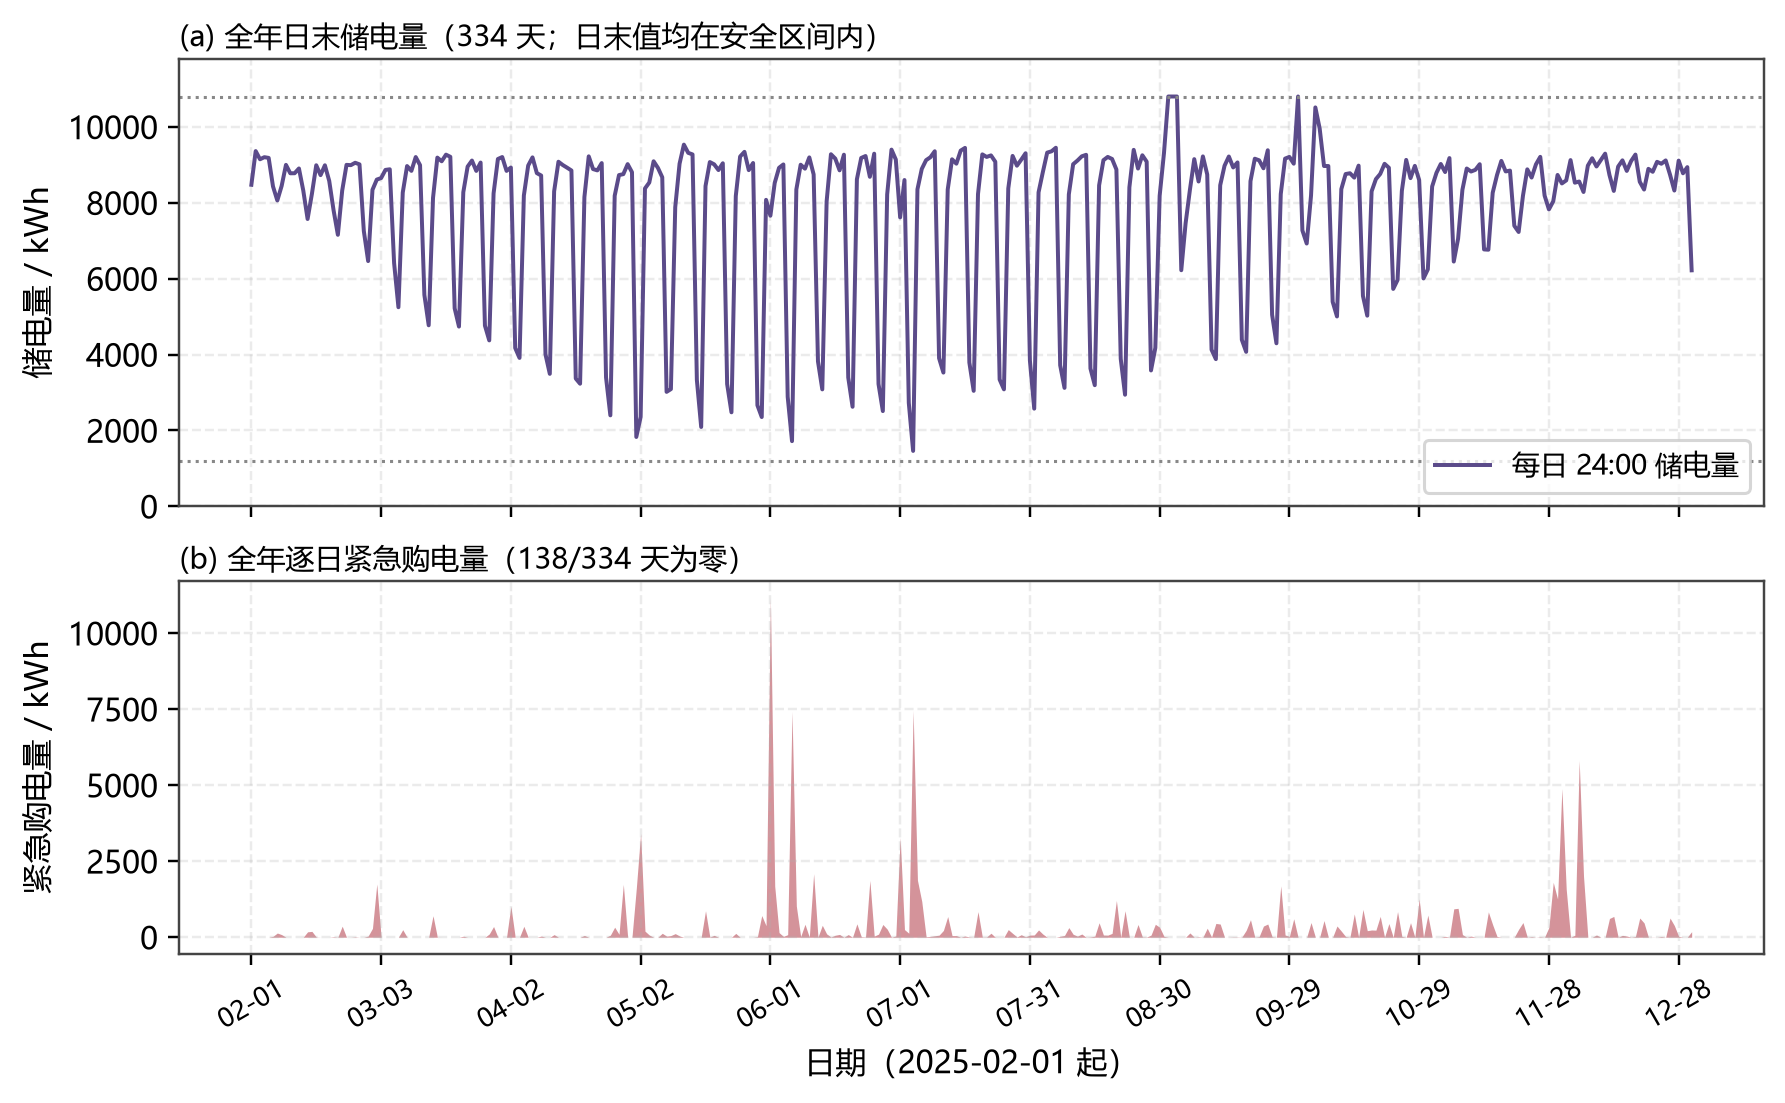
\includegraphics[width=0.82\textwidth]{figures/fig_q2_year.png}
  \caption{问题二：全年日末储电量与逐日紧急购电量}
  \label{fig:q2year}
\end{figure}

由上述结果可以得出以下结论：

\begin{enumerate}[itemsep=1pt, topsep=2pt]
  \item 计划层“多买”换来了执行层“少补”。在同一严格储电量执行层下，
        本文方案比点预测方案（负荷取同星期几均值、光伏取近 7 天均值）的总费低
        2\,280\,994 元（13\,846\,553 元对 16\,127\,547 元），说明在 $5$ 倍紧急电价下，
        计划层的正偏置是有价值的。
  \item 储电量全程受控。全年实际执行储电量始终落在 $[1200,10800]$ kWh 内，
        未出现越界。
  \item 紧急购电高度集中。334 天中有 138 天完全没有触发紧急购电，紧急购电只分布在
        196 天、共 311 个连续时间段。
\end{enumerate}



\subsection{问题三：考虑分位对冲与场景化日内调整的两阶段随机优化模型}
\label{sec:q3model}

\subsubsection{模型结构：四层因果}

问题三的核心是\emph{信息结构}：每天 0:00 依据附件 3 第 0 档预报制定计划，6:00、
12:00、18:00 三个时刻再依据新发布的预报\emph{调整}计划。由 \S2.4 之(2) 已推出
违约费恒为零，即调整只允许上调。据此，本文将模型组织为计划、调整、执行与结算
四层因果结构，如表 \ref{tab:q3layer} 所示。

\begin{table}[!htbp]
  \centering
  \caption{问题三模型的四层因果结构}\label{tab:q3layer}
  \zihao{-5}
  \begin{tabular}{@{}l l l l@{}}
    \toprule[1.5pt]
    \hd{层} & \hd{时刻} & \hd{决策} & \hd{用到的信息}\\
    \midrule[1pt]
    计划层 & 每天 0:00 & $\hat g$（144 槽）$+$ 逐情景 $c_\omega,d_\omega,e_\omega$
      & 第 0 档预报 $+$ 分组负荷基线 $+$ 同组历史日\\
    调整层 & 6:00 / 12:00 / 18:00 & 把后续时窗的目标净需求上调
      & 该时刻新发布的预报 $+$ 当天已发生时段的实测\\
    执行层 & 逐槽（10 min） & 跟随计划充放电、必要时强制补放
      & 实测负载与光伏、当前储电量\\
    结算层 & 事后 & 按式 \eqref{eq:q3cost} 结算 & 实测轨迹\\
    \bottomrule[1.5pt]
  \end{tabular}
\end{table}

\subsubsection{第一层：0:00 计划模型}

计划层由两部分构成：一是可靠性垫层，把预报净需求的误差分布的分位数垫在
目标上；二是\emph{两阶段}日前套利规划，在 144 槽上联合解出计划购电量与
逐情景的充放电量。后者是提升效益的主要来源：题面开篇即认可在电价较低或
分布式能源有剩余电量的时间段为储能设备充电、在电价较高的时间段释放电能。
实测日均充电量为 18\,306 kWh，往返效率 $d/\eta\div c=\eta^2=0.81$。

计划层不按预报净需求的均值购买，而按分位数购买；且\textbf{只有计划购电量
$\hat g$ 是 0:00 拍板的承诺量}，充放电 $c,d$、紧急购电量 $e$ 与储电量 $S$
都降为逐情景 $\omega$ 的追索变量（情景集取同组历史日，与问题二同思路）。
这样电池自己按情景对冲、承诺量按情景分布取分位，而不是让一个数同时干两件事。
其优化模型如下所示：

\begin{equation}
\begin{gathered}
\min\; Z_3^{\text{plan}}=\sum_t p_t\hat g_t\Delta t
  +\frac{1}{K}\sum_\omega\sum_t 5p_t e_{\omega,t}\Delta t\\[2pt]
\text{s.t.}\quad(\text{逐情景 }\omega=1,\dots,K)\;
\begin{cases}
S_{\omega,t+1}=S_{\omega,t}+\eta c_{\omega,t}\Delta t-\dfrac{d_{\omega,t}\Delta t}{\eta},
  & \text{（储电递推）}\\
c_{\omega,t}-d_{\omega,t}\le\hat g_t-N_{\omega,t}, & \text{（充电只吃富余）}\\
d_{\omega,t}+e_{\omega,t}\ge N_{\omega,t}-\hat g_t, & \text{（负荷必须供上）}\\
S^{\min}\le S_{\omega,t}\le S^{\max} & \text{（电量区间）}\\
S_{\omega,0}=S_0,\; S_{\omega,T}=6000 & \text{（日末锚点）}\\
0\le c_{\omega,t},d_{\omega,t}\le P_{\max},\; \hat g_t\ge0,\; e_{\omega,t}\ge0,
  & \text{（功率与非负）}
\end{cases}\\[2pt]
N_{\omega,t}=L_{\omega,t}-P_{\omega,t}+h_t,\; h_t=Q_{\tau(t)}\bigl(\mathrm{resid}_t\bigr),\;
t=0,1,\dots,143
\end{gathered}
\label{eq:q3plan}
\end{equation}

式中 $N_{\omega,t}$ 为第 $\omega$ 个历史同组日的净需求叠加可靠性垫层后的目标
净需求：$h_t$ 是残差 $\mathrm{resid}_t$（实际净需求减该档预报净需求）在分位
$\tau(t)$ 处的经验分位数，它对准的是\emph{毛净需求} $L-P$（若对准“电池放完后的
残余缺口”会把放电算两遍，计划据此少买、紧急购电暴涨）。式中逐 10 分钟粒度的光伏
预报，由附件 3 的整点预报按 \S2.6 之(3) 的\textbf{线性插值}给出（若按分段常数保持，
正午峰值会被削成台阶）。$S_0$ 取当日实测起始
储电量，$S_T=6000$ 是自加假设（假设 7）。购电功率按题面字面读法\textbf{不设上界}
（附录 1 只给出储能的最大充放电功率）。对冲分位按 \S2.4 之(3)分块设定：
第 0 块（盲窗）取 $\tau_0\approx0.55$，后三块（可调段）取 $\tau'\approx0.42$，
两者的取值由数值扫描确定（见 §\ref{sec:q3result}）。

\subsubsection{第二层：日内调整模型}

在 6:00、12:00、18:00 各解一次调整模型，决策变量为调整购电量 $g$、充放电 $c,d$、
储电量 $SOC$，目标是修正后续时窗的目标净需求。其关键机制是水平校正：
预报误差中“整天整体偏高/偏低”那一支是强自相关的，仅取残差分位数抓不到，必须用当天
已发生时段的实测负荷与基准负荷之比直接测出，再按该比值缩放剩余时段的预报。

调整模型按如下步骤求解：

\begin{enumerate}[label=Step \arabic*., leftmargin=*, itemsep=2pt, topsep=3pt]
  \item 推进储电量。用已定策略与实际发生的负载、光伏，按储能递推式把储电量
        推进到当前调整时刻；
  \item 计算水平校正比值。令
        $r=\bigl(\sum_{t<a}L_t\bigr)\big/\bigl(\sum_{t<a}L^{\text{base}}_t\bigr)$，
        其中 $a$ 为当前调整时刻对应的槽号；
  \item 校正目标净需求。对剩余时窗 $[a,b)$ 取
        $N^{\text{cor}}=r\,L^{\text{base}}_{[a,b)}-\hat P_{[a,b)}$，
        并对历史残差施以同样的校正，得到校正后的残差分布 $R^{\text{cor}}$；
  \item 求解并只允许上调。令
        $N_t^{\text{adj}}\leftarrow\max\bigl(N_t^{\text{adj}},\
        N_t^{\text{cor}}+Q_{\tau'}(R^{\text{cor}})\bigr)$，
        据此重解剩余时段的购电量与充放电量；
  \item 执行至下一调整时刻。按所得策略执行，直至下一个调整时刻或当日结束。
\end{enumerate}

\subsubsection{模型求解}
\label{sec:q3result}

定稿配置为 $\tau_0=0.55$、$\tau'=0.42$、三档调整全开、水平校正开启、
购电功率按题面字面读法不设上界。求解与自检的检查项列于表 \ref{tab:q3check}。

\begin{table}[!htbp]
  \centering
  \caption{问题三求解结果的检验}\label{tab:q3check}
  \zihao{-5}
  \begin{tabular}{l l l}
    \toprule[1.5pt]
    \hd{检验项} & \hd{期望} & \hd{实测}\\
    \midrule[1pt]
    违约费 $=0$（\S2.4 之(2) 的推论） & 0 & 0.00 元 $\checkmark$\\
    结果 $\ge$ 完美预见下界 & $\ge$ 12\,229\,461 & 13\,630\,568 元 $\checkmark$\\
    储能能量守恒 & $d/\eta\div c=\eta^2$ & $5\,370\,112/6\,629\,038=0.8101$ $\checkmark$\\
    真实储电量轨迹 & 落在 $[1200,10800]$ & 打满上下限，0 越界 $\checkmark$\\
    调整层不泄漏到第 0 块 & 变化 0 kWh & 0 kWh $\checkmark$\\
    写盘费 $=$ 结算值 & 相等 & 差 0.0000 元 $\checkmark$\\
    \bottomrule[1.5pt]
  \end{tabular}
\end{table}

本文还用一份\emph{不引用任何求解器}的独立脚本，从附件 1/2 重读原始数据、
再把交付的 \texttt{result3.xlsx} 读回来重算：124 个无紧急购电日的费用精确对账，
最大残差 0.005225 元；储电量递推残差 $3\times10^{-4}$ kWh，跨日衔接 0.0000 kWh；
全年合计 13\,630\,567.82 元。交付文件可被第三方按同一口径独立核出。

\subsubsection{求解结果与参数确定}

\noindent（1）总体结果。表 \ref{tab:q3summary} 给出统计窗口
2025.2.1--12.31（334 天）的总体结果。

\begin{table}[!htbp]
  \centering
  \caption{问题三求解结果的总体汇总（窗口 2/1--12/31）}\label{tab:q3summary}
  \zihao{-5}
  \begin{tabular}{l r l}
    \toprule[1.5pt]
    \hd{指标} & \hd{数值} & \hd{单位}\\
    \midrule[1pt]
    计划购电量 $\sum\hat g_t\Delta t$ & 20\,587\,054 & kWh\\
    最终调整购电量 $\sum g_t\Delta t$ & 21\,411\,743 & kWh\\
    紧急购电量 $\sum e_t\Delta t$     & 49\,632      & kWh\\
    \midrule[1pt]
    计划购电费 $\sum p\hat g\Delta t$ & 12\,553\,713 & 元\\
    违约费 $0.5\sum p(\hat g-g)^{+}\Delta t$ & 0 & 元\\
    超额费 $1.5\sum p(g-\hat g)^{+}\Delta t$ & 794\,737 & 元\\
    紧急购电费 $5\sum p e\Delta t$    & 282\,118     & 元\\
    \midrule[1pt]
    总购电费 $Z_3$ & 13\,630\,568 & 元\\
    \midrule[1pt]
    储能充电 / 放电 & 6\,629\,038 / 5\,370\,112 & kWh\\
    真实储电量日内轨迹区间 & $[1\,200,\ 10\,800]$ & kWh\\
    年末储电量 & 5\,760 & kWh\\
    完美预见下界（同口径，无上界读法） & 12\,229\,461 & 元\\
    \bottomrule[1.5pt]
  \end{tabular}
\end{table}

相对同口径完美预见下界 12\,229\,461 元高出 $11.46\%$，即预报误差的代价约 140 万元。

\noindent（2）指定日期的结果。表 \ref{tab:q3t1} 按题目表 1 的格式给出四个
指定日期的购电量（数据源为最终执行的调整购电量 $g$），表 \ref{tab:q3t2}、表
\ref{tab:q3t3} 分别给出储能设备充放电量与紧急购电量。

\begin{table}[!htbp]
  \centering
  \caption{问题三：微网在指定日期的购电量及全天购电量和购电费}
  \label{tab:q3t1}
  \zihao{-5}
  \begin{tabular}{c c c c c c c}
    \toprule[1.5pt]
    \hd{日期} & \hd{时间段} & \hd{购电量/kWh} & \hd{时间段} & \hd{购电量/kWh} & \hd{时间段} & \hd{购电量/kWh}\\
    \midrule[1pt]
    2025.3.20 & 10:00-10:10 & 0.00 & 12:00-12:10 & 709.08 & 14:00-14:10 & 0.00\\
     & 16:00-16:10 & 658.11 & 18:00-18:10 & 693.59 & 20:00-20:10 & 0.00\\
    \multicolumn{6}{l}{\hd{全天购电量 73\,194.30 kWh；全天购电费 45\,514.34 元}}\\
    \midrule[1pt]
    2025.6.21 & 10:00-10:10 & 0.00 & 12:00-12:10 & 0.00 & 14:00-14:10 & 0.00\\
     & 16:00-16:10 & 166.11 & 18:00-18:10 & 0.00 & 20:00-20:10 & 0.00\\
    \multicolumn{6}{l}{\hd{全天购电量 34\,243.72 kWh；全天购电费 19\,438.90 元}}\\
    \midrule[1pt]
    2025.9.23 & 10:00-10:10 & 0.00 & 12:00-12:10 & 373.50 & 14:00-14:10 & 0.00\\
     & 16:00-16:10 & 580.23 & 18:00-18:10 & 741.78 & 20:00-20:10 & 0.00\\
    \multicolumn{6}{l}{\hd{全天购电量 67\,252.91 kWh；全天购电费 42\,615.05 元}}\\
    \midrule[1pt]
    2025.12.21 & 10:00-10:10 & 0.00 & 12:00-12:10 & 952.41 & 14:00-14:10 & 0.00\\
     & 16:00-16:10 & 845.85 & 18:00-18:10 & 680.36 & 20:00-20:10 & 0.00\\
    \multicolumn{6}{l}{\hd{全天购电量 94\,985.55 kWh；全天购电费 61\,645.25 元}}\\
    \bottomrule[1.5pt]
  \end{tabular}
\end{table}

\begin{table}[!htbp]
  \centering
  \caption{问题三：储能设备在指定日期的充放电量及 0:00 和 24:00 的储电量}
  \label{tab:q3t2}
  \zihao{-5}
  \begin{tabular}{c c c c c c c}
    \toprule[1.5pt]
    \hd{日期} & \hd{时间段} & \hd{充电量/kWh} & \hd{放电量/kWh} & \hd{时间段} & \hd{充电量/kWh} & \hd{放电量/kWh}\\
    \midrule[1pt]
    2025.3.20 & 0:00-4:00 & 4462.84 & 157.90 & 4:00-8:00 & 962.93 & 5148.01\\
    & 8:00-12:00 & 6291.46 & 2777.38 & 12:00-16:00 & 3751.11 & 254.72\\
    & 16:00-20:00 & 13.46 & 5701.84 & 20:00-24:00 & 5530.01 & 3055.96\\
    & \multicolumn{2}{l}{\hd{0:00 储电量 6142.95}} & \multicolumn{3}{l}{\hd{24:00 储电量 6058.23}}\\
    \midrule[1pt]
    2025.6.21 & 0:00-4:00 & 341.52 & 529.15 & 4:00-8:00 & 451.95 & 4412.75\\
    & 8:00-12:00 & 10097.91 & 0.00 & 12:00-16:00 & 0.00 & 0.00\\
    & 16:00-20:00 & 66.98 & 5827.72 & 20:00-24:00 & 5803.88 & 2614.38\\
    & \multicolumn{2}{l}{\hd{0:00 储电量 6488.76}} & \multicolumn{3}{l}{\hd{24:00 储电量 6703.67}}\\
    \midrule[1pt]
    2025.9.23 & 0:00-4:00 & 4425.75 & 119.89 & 4:00-8:00 & 806.02 & 6400.55\\
    & 8:00-12:00 & 4579.77 & 1896.62 & 12:00-16:00 & 6029.95 & 403.62\\
    & 16:00-20:00 & 70.62 & 5851.17 & 20:00-24:00 & 5494.14 & 2878.80\\
    & \multicolumn{2}{l}{\hd{0:00 储电量 6343.41}} & \multicolumn{3}{l}{\hd{24:00 储电量 6108.32}}\\
    \midrule[1pt]
    2025.12.21 & 0:00-4:00 & 4846.83 & 59.72 & 4:00-8:00 & 1722.31 & 1612.87\\
    & 8:00-12:00 & 5495.52 & 7648.87 & 12:00-16:00 & 7861.60 & 2330.15\\
    & 16:00-20:00 & 25.29 & 5833.71 & 20:00-24:00 & 5385.34 & 2893.42\\
    & \multicolumn{2}{l}{\hd{0:00 储电量 5812.58}} & \multicolumn{3}{l}{\hd{24:00 储电量 5972.75}}\\
    \bottomrule[1.5pt]
  \end{tabular}
\end{table}

\begin{table}[!htbp]
  \centering
  \caption{问题三：微网在指定日期的紧急购电量}
  \label{tab:q3t3}
  \zihao{-5}
  \begin{tabular}{l l r}
    \toprule[1.5pt]
    \hd{日期} & \hd{紧急购电时间段} & \hd{紧急购电量/kWh}\\
    \midrule[1pt]
    2025.3.20 & 21:30-21:50 & 33.8123\\
     & \hd{当日合计} & \hd{33.81}\\
    \midrule[1pt]
    2025.6.21 & ——（当日无紧急购电） & 0.0000\\
     & \hd{当日合计} & \hd{0.00}\\
    \midrule[1pt]
    2025.9.23 & 20:20-20:30 & 6.3750\\
     & 20:50-21:00 & 59.5433\\
     & \hd{当日合计} & \hd{65.92}\\
    \midrule[1pt]
    2025.12.21 & 20:30-20:50 & 22.3085\\
     & 21:30-21:50 & 46.4903\\
     & \hd{当日合计} & \hd{68.80}\\
    \bottomrule[1.5pt]
  \end{tabular}

  \vspace{2pt}
  \parbox{0.95\textwidth}{\zihao{-5} 注：购电量单位为 kWh，四个指定日期合计 168.53 kWh。}
\end{table}

\noindent（3）按 6 小时时窗的调整结构。把全年 334 天按四个发布时刻切成
6 小时时窗后，各窗的计划量与最终调整量对照如图 \ref{fig:q3win}(a)，逐日净调整量的
时窗构成如图 \ref{fig:q3win}(b)。据此可得出三条结论：

\begin{figure}[!htbp]
  \centering
  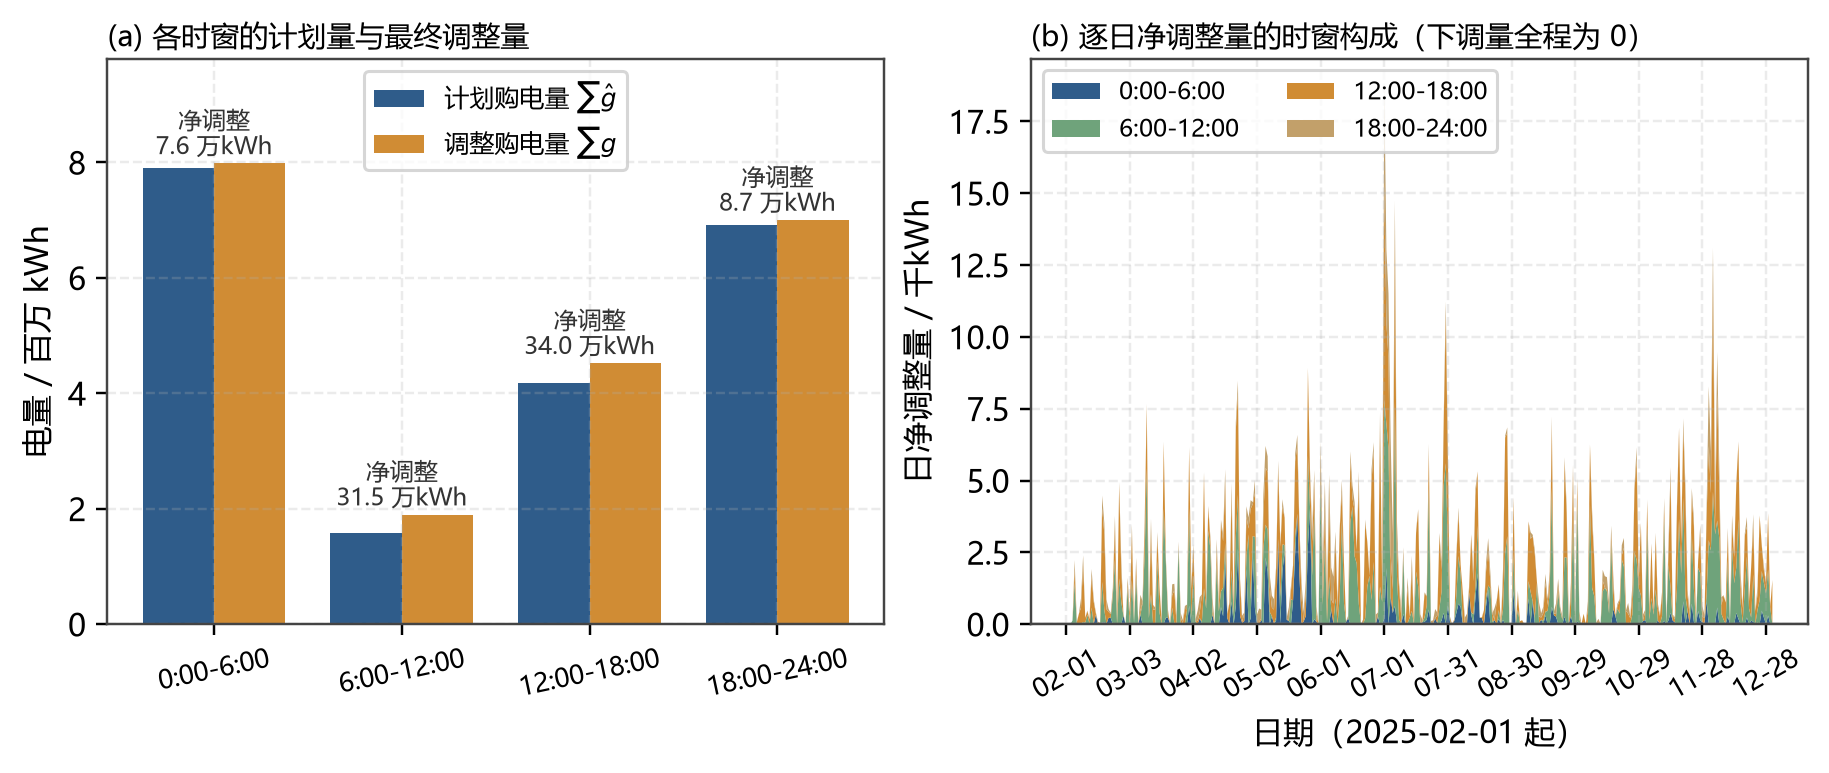
\includegraphics[width=0.99\textwidth]{figures/fig_q3_windows.png}
  \caption{问题三：按 6 小时时窗的计划量与调整量}
  \label{fig:q3win}
\end{figure}

\begin{enumerate}[itemsep=1pt, topsep=2pt]
  \item 调整在电量口径上也是单边向上的：四个时窗的下调量\emph{全部为 0}，
        年净调整量 824\,689 kWh 全部来自上调。这是 \S2.4 之(2) 那条推论的直接实证。
  \item 调整量集中在两个可调时窗：6:00--12:00 为 31.71 万 kWh、
        12:00--18:00 为 34.08 万 kWh，两者合计占净调整总量的 $79.8\%$；
        而 0:00--6:00 虽计划量最大（790.81 万 kWh），净调整仅 7.54 万 kWh（$9.1\%$），
        这正是盲窗无调整机会在电量上的体现。
  \item 紧急购电量集中在入夜后：18:00--24:00 为 37\,449 kWh、6:00--12:00 为
        10\,584 kWh、12:00--18:00 为 0，盲窗仅 1\,598 kWh。
        说明在可调时窗内调整通道已把缺口基本补齐。
\end{enumerate}

\noindent（4）对冲分位是平台中心，不是尖点最优。图 \ref{fig:q3tau} 给出两条一维扫描：
$\tau'$ 的两端都翘起来（$\tau'=0.10$ 时紧急购电 471\,422 kWh，比定稿高 9.5 倍，
调整层形同关闭），$\tau_0$ 同样在中间取到最优。

\begin{figure}[!htbp]
  \centering
  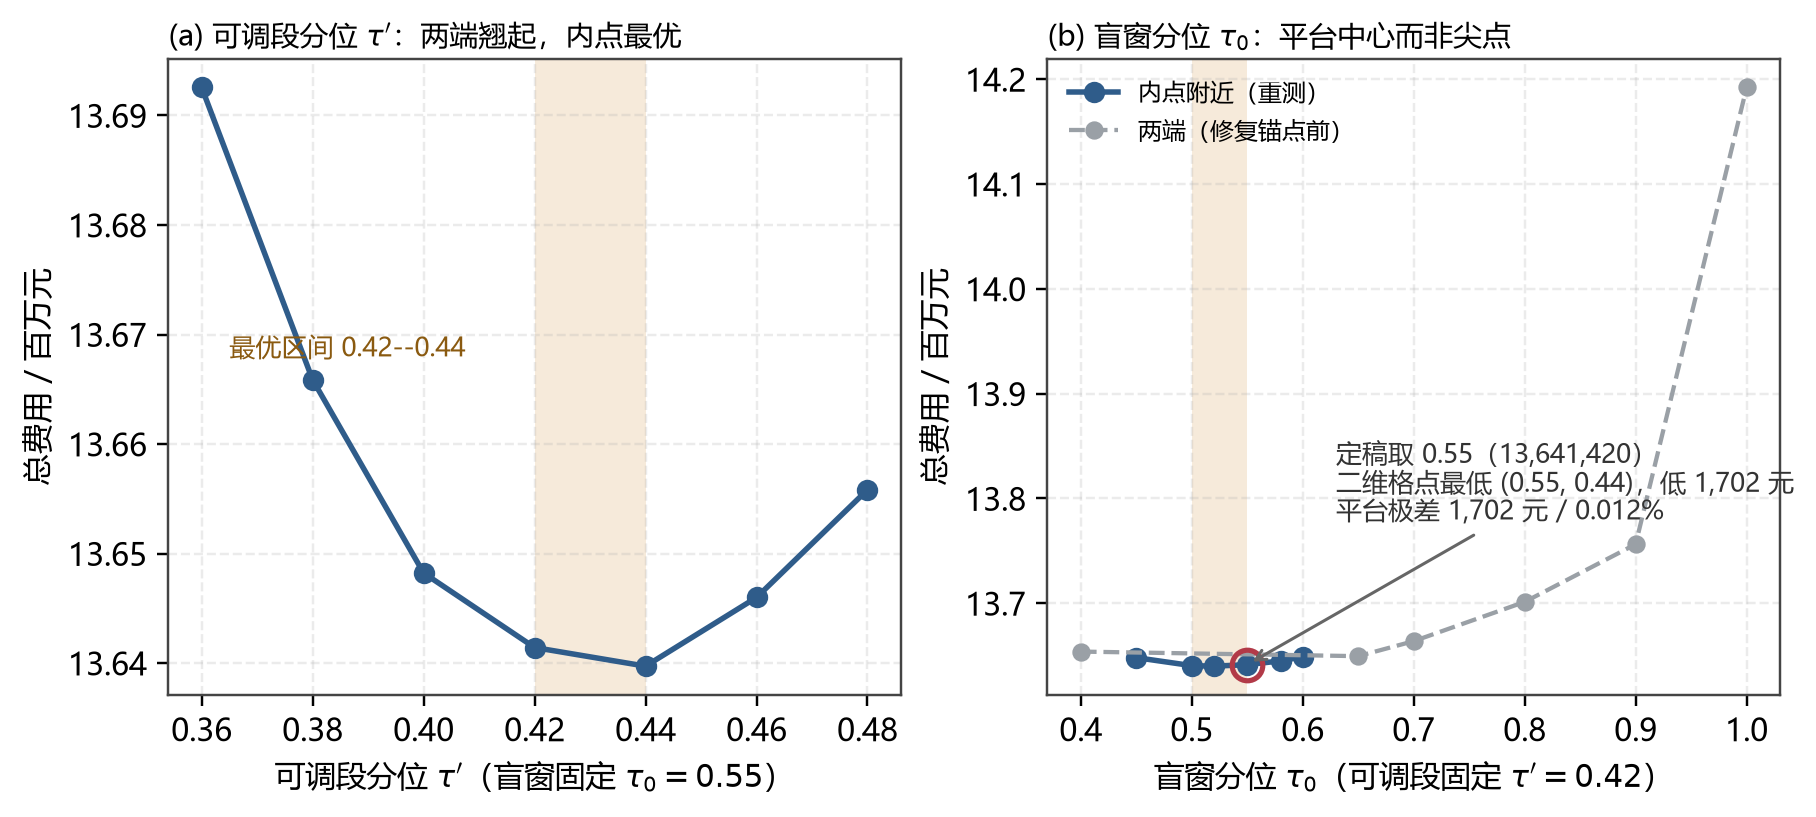
\includegraphics[width=0.99\textwidth]{figures/fig_tau.png}
  \caption{对冲分位的敏感性}
  \label{fig:q3tau}
\end{figure}

曲面在最优附近是一个\emph{宽平台}：$\tau_0\in[0.50,0.55]\times\tau'\in[0.42,0.44]$
的极差仅 2\,296 元（$0.017\%$）；网格最小值落在 $(0.52,0.42)$，比定稿仅低
1\,382 元（$0.010\%$）——为不过拟合扫描网格，定稿取 $(\tau_0,\tau')=(0.55,0.42)$。
因此本文的表述是“平台中心是 $(0.55,0.42)$”，而\emph{不声称}求得尖点最优。

\textbf{分位必须随计划层重调}：确定性计划层时代调出的 $(0.80,0.55)$ 原样搬到
追索版会偏贵 185\,974 元。以固定 $\tau_0$ 的一维扫描为例，$\tau'$ 由 $0.55$ 下调到
$0.42$ 时，计划购电费减少 48.4 万元（少承诺），代价是超额费 $+10.6$ 万元、
紧急购电费 $+18.6$ 万元，三项净省 19.2 万元。方向与 \S2.4 之(3) 一致：计划层
自己按情景对冲后，调整层就不该再叠加一层厚缓冲；$0.42$ 也比旧值 $0.55$ 更接近
静态理论值 $1/3$。

\noindent（5）消融实验。图 \ref{fig:q3ablation} 给出逐块关闭后的总费用，
并以完美预见下界作参照。

\begin{figure}[!htbp]
  \centering
  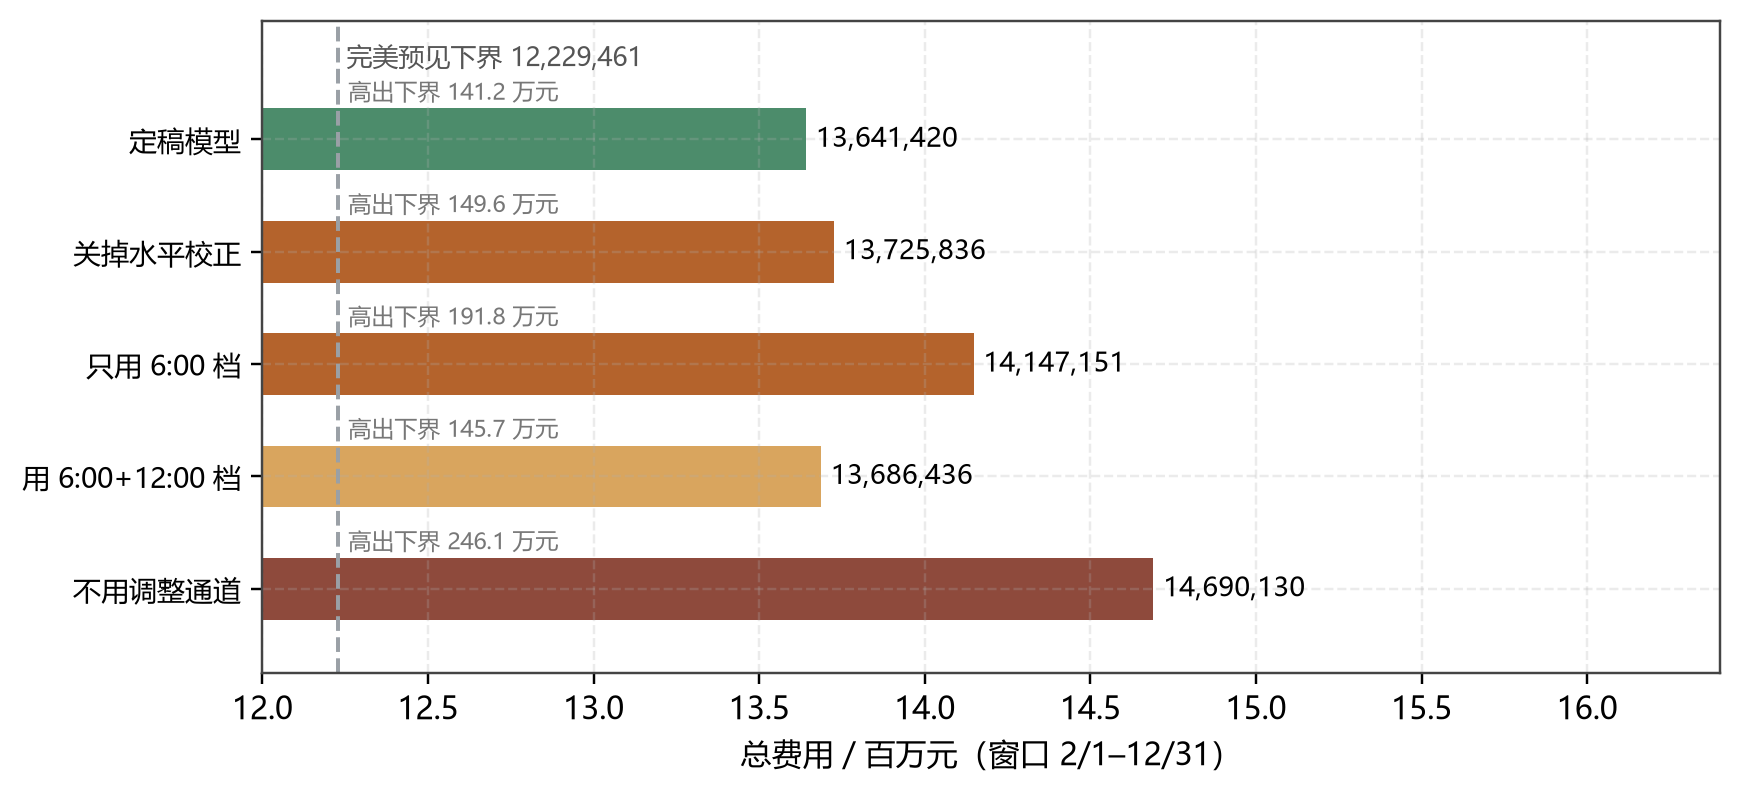
\includegraphics[width=0.90\textwidth]{figures/fig_q3_ablation.png}
  \caption{问题三的消融实验}
  \label{fig:q3ablation}
\end{figure}

由此得出三条结论：

\begin{enumerate}[itemsep=1pt, topsep=2pt]
  \item 日内调整通道是价值最大的一块：关闭后总费升至 14\,690\,130 元，
        即该通道值 105.96 万元，其中 6:00 档 54.46 万元、12:00 档
        46.05 万元、18:00 档 5.45 万元；
  \item 调整层的水平校正值 8.04 万元：只取残差分位数而不做水平校正，
        会漏掉“整天整体偏高/偏低”那一支自相关误差；
  \item 18:00 档只值 5.45 万元（占 $0.40\%$），比确定性计划层时代的 3\,865 元
        高一个量级——追索计划层把前两档能吃掉的误差吃完了，留给 18:00 档的反而更多。
        这与附件 3 的预报质量分析方向一致（见下节）。
\end{enumerate}

\noindent（6）基线口径的归因。低需求日分组带来的 61.04 万元增益与调整通道的
105.96 万元\emph{不可相加}，因为两者在修同一类偏差，是部分替代品。这也是水平校正的
边际估值从确定性计划层时代的 13.30 万元降到追索版的 8.04 万元的原因：计划层自己
按情景对冲后，基线口径已经吸收了当初水平校正要修的那部分偏差。

\subsubsection{是否需要引入其他时刻的预报}

题面要求分析是否需要引入其他时刻的预报。判据是：一份新预报有没有价值，看它能否
\emph{降低净需求（负荷减光伏）的预报误差}。图 \ref{fig:q3rmse} 给出逐档、逐时窗的
净需求预报 RMSE。

\begin{figure}[!htbp]
  \centering
  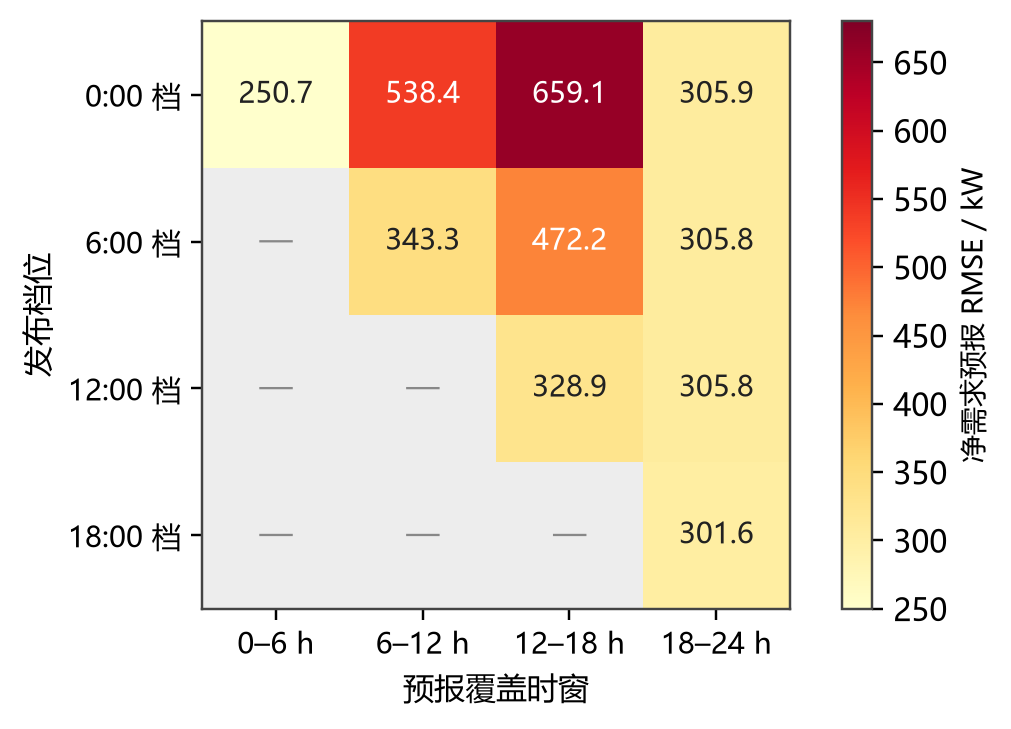
\includegraphics[width=0.68\textwidth]{figures/fig_q3_rmse.png}
  \caption{各发布档、各时窗的净需求预报 RMSE 矩阵}
  \label{fig:q3rmse}
\end{figure}

逐档增量分析表明：引入 6:00 档把上午净需求的误差从 538.4 kW 降到 343.3 kW
（$-36.2\%$）；引入 12:00 档把午后误差从 659.1 kW 降到 328.9 kW（$-50.1\%$）；
而引入 18:00 档对 18--24 h 的误差只从 305.8 kW 降到 301.6 kW（$-1.4\%$）。因此：

\begin{enumerate}[itemsep=1pt, topsep=2pt]
  \item 需要引入 6:00 档，把上午的净需求误差降低 $36.2\%$，在成本口径下
        值 54.46 万元；
  \item 需要引入 12:00 档，把午后的误差降低 $50.1\%$，值 46.05 万元；
  \item 18:00 档可以省掉，因为该时窗已入夜、光伏接近 0，而 0:00 档对夜间净需求
        本来就报得不错（305.9 kW），18:00 档没有带来实质新信息。按成本口径其边际
        价值仅 5.45 万元（$0.40\%$），可省，但并非无价值。
\end{enumerate}

\noindent 电量口径给出一个补充观察：盲窗（0:00--6:00）虽无调整机会，其紧急购电仅
1\,598 kWh，反而远低于 18:00--24:00 的 37\,449 kWh（也低于 6:00--12:00 的
10\,584 kWh）。原因是两段采用了不同的对冲水位：盲窗按 $\tau_0\approx0.55$ 正偏对冲、
买得更足，可调时窗按 $\tau'\approx0.42$ 买入，残余缺口交由 $1.5p$ 的调整通道在
6:00/12:00/18:00 消化，而不是留给 $5p$ 的紧急购电。

\noindent 一处补充口径。附件 3 的 0:00 档\emph{并不比历史
统计预测更准}：在光伏口径上，0:00 档的 RMSE 为 383.0 kW，反而差于“近 7 天均值”的
303.9 kW。真正变准的只有 6:00、12:00 两档。本文因此不把附件 3 描述为全面优于统计
预测的信息源。



\subsection{问题四：波动电价下的购电策略模型}
\label{sec:q4model}

\subsubsection{模型建立}

问题四把常量电价 $p_t$ 替换为附件 4 的逐日逐槽实际电价 $p_{d,t}$。由 \S2.5 的分析，
建模上需要改动的只有价格的进入方式，其余（储能物理、决策变量边界、$\gamma$ 可交付
结构、口径 A 的四项结算、334 天窗口）全部沿用。

\noindent（1）价格的两个进入点。模型中有两个价格向量，分工不可混用：
计划层的价格系数取“公布的分时电价剖面”（部分信息口径，即 0:00 不知道当天实际
电价），或取“当天实际电价”（完全信息口径，作为下界与敏感性）；结算层与写盘层
一律使用附件 4 的实际价。价格整体缩放 $\pm30\%$ 时，由式 \eqref{eq:q3cost} 可知
四项费用都按同一比例缩放，因此账单是价格的\emph{线性}函数。

\noindent（2）问题四-三与问题三同构。在部分信息口径下，计划层的目标函数、
滚动调整的窗口价以及结算层以外的各个环节，都退化为当天的单一价格剖面，与问题三
完全一致。因此问题四-三的模型即问题三模型加上价格的结算口径，数学表达仍为
式 \eqref{eq:q3cost}--\eqref{eq:q3plan}，只是结算层的 $p_t$ 换成 $p_{d,t}$。

\noindent（3）问题四-二：场景集需联合价格与净负荷。问题三的场景集只依赖
附件 3 的光伏预报档位，与价格不联动；而问题四需要“缺口时段电价更高”这条渠道进入
模型，因此把紧急购电的场景系数由标量 $5p$ 改为逐场景逐槽
$5\,p_{\omega,t}/K$。这一改动让\emph{价格与缺口的联合分布}直接参与决策，
因此问题四-二的策略确实不同于问题二（\S\ref{sec:q4result} 表
\ref{tab:q4summary}）。

\subsubsection{模型求解}

求解步骤与问题三相同（计划层 LP $\to$ 三个时刻的水平校正与上调 $\to$ 逐槽执行
$\to$ 按式 \eqref{eq:q3cost} 结算），差别只在价格进入方式（部分信息口径）与写盘价格
（附件 4 实际价）。流程如图 \ref{fig:q4flow} 所示。

\begin{figure}[!htbp]
  \centering
  \begin{tikzpicture}[node distance=6.5mm and 6mm]
    \node[databox] (a) {附件 4\\逐日逐槽实际电价};
    \node[databox, below=of a] (b) {附件 1\\公布的分时电价剖面};
    \node[box, right=of b, yshift=6mm] (c) {计划层 LP\\价格预期（部分信息口径）};
    \node[box, right=of c] (d) {6/12/18 点\\水平校正 $+$ 只上调};
    \node[box, below=of d] (e) {逐槽执行\\严格储电量因果策略};
    \node[box, left=of e] (f) {结算层\\按附件 4 实际价结算};
    \node[resbox, left=of f] (g) {输出 result4-3.xlsx\\result4-2.xlsx};
    \draw[ar] (a) -- (c);
    \draw[ar] (b) -- (c);
    \draw[ar] (c) -- (d); \draw[ar] (d) -- (e);
    \draw[ar] (a) -- (f);
    \draw[ar] (e) -- (f); \draw[ar] (f) -- (g);
  \end{tikzpicture}
  \caption{问题四的求解流程}
  \label{fig:q4flow}
\end{figure}

\subsubsection{求解结果}
\label{sec:q4result}

\noindent（1）波动电价不改变最优策略，只改变账单。计划层的价格系数取\emph{公布的分时
电价剖面}、不使用当天实际价，因此换价后购电量、充放电量与紧急购电量逐元素不变，
变化的只有按实际价结算的账单；同一决策下账单是价格水平的线性函数，将\emph{价格整体
缩放} $\pm30\%$（13 档）后策略同样逐元素不变，账单精确线性，最大偏差
$\max|Z(s)-sZ(1)|=0.000000$ 元。

\begin{quote}\zihao{-5}
\textbf{基准备注}：本节各绝对数值由问题四的两个交付文件给出，它们与问题三\emph{前一版}
基准（确定性计划层 $+$ $G\le5000$ kW）同源。问题三本轮已改为追索计划层 $+$ 无上界
读法，两项交付文件需按新基准重出后本节绝对数随之更新；\textbf{方向性结论}
（波动电价只改账单不改决策、交付表富余丢弃是继承性质、两条负结果）\textbf{不受影响}。
\end{quote}

这一结论与 \S2.5 的方差分解互为印证：计费公式 \eqref{eq:q3cost} 的四项收费都是
同一个 $p$ 的倍数，而附件 4 中占主导的日水平因子 $a_d$ 是全天均匀平移，
\emph{均匀平移不改变任何边际权衡}。图 \ref{fig:q4shift} 把附件 4 的最低价日、
中位价日与最高价日同附件 1 基准剖面画在一起：三条曲线的形状一致，去掉各自的日均价
后基本重合，差别只来自占 $6.2\%$ 的日内残差。

\begin{figure}[!htbp]
  \centering
  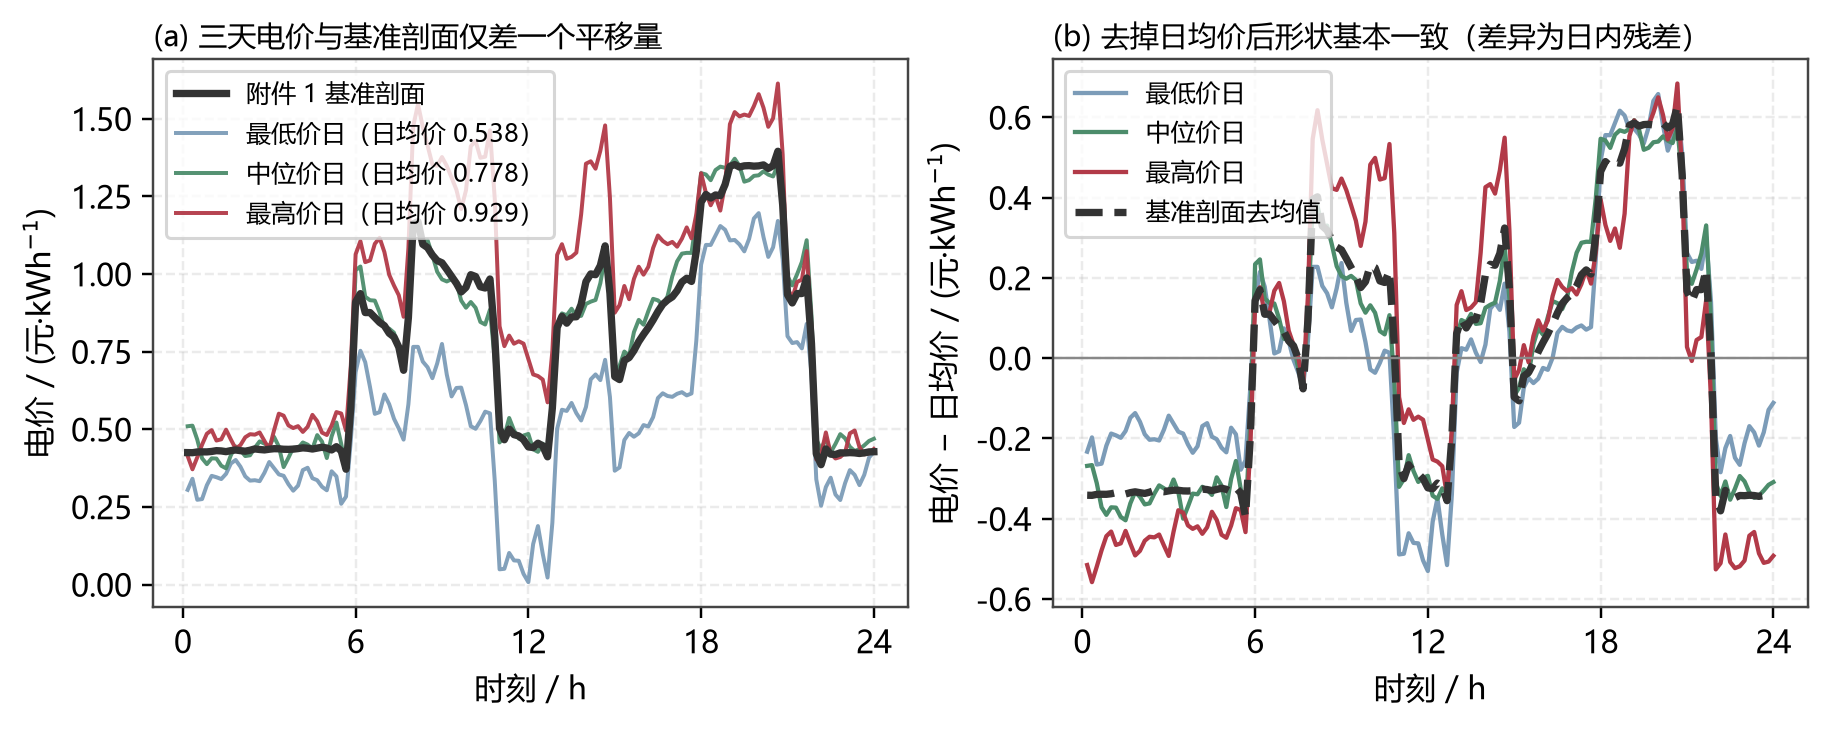
\includegraphics[width=0.99\textwidth]{figures/fig_q4_shift.png}
  \caption{附件 4 的代表性日与基准剖面}
  \label{fig:q4shift}
\end{figure}

\noindent（2）总体结果。表 \ref{tab:q4summary} 给出两个交付文件的汇总。

\begin{table}[!htbp]
  \centering
  \caption{问题四两个交付文件的总体结果（窗口 2/1--12/31）}\label{tab:q4summary}
  \zihao{-5}
  \begin{tabular}{l r r}
    \toprule[1.5pt]
    \hd{指标} & \hd{result4-3（对应问题三）} & \hd{result4-2（对应问题二）}\\
    \midrule[1pt]
    总费用 / 元 & 15\,007\,661 & 14\,736\,353\\
    　计划购电费 & 13\,902\,153 & 14\,206\,059\\
    　违约费 & 0 & 0\\
    　超额费 & 720\,462 & 其余两项合计 530\,293\\
    　紧急购电费 & 385\,046 & \\
    　紧急购电量 / kWh & 76\,784 & ——\\
    计划购电量 $\sum\hat g$ / kWh & 20\,795\,914 & 21\,637\,974\\
    实际购电量 $\sum g$ / kWh & 21\,424\,459 & ——\\
    储能充电 / 放电 / kWh & 6\,114\,270 / 4\,953\,300 & 5\,813\,976 / 4\,708\,500\\
    真实储电量区间 / kWh & $[1\,200,\ 10\,800]$ & $[1\,200,\ 10\,800]$\\
    年末储电量 / kWh & 4\,811 & 5\,263\\
    完美预见下界（同口径）/ 元 & 13\,014\,628 & 13\,014\,628\\
    \bottomrule[1.5pt]
  \end{tabular}
\end{table}

问题四-三相对问题三的账单变化为 $+721\,930$ 元（$\times1.0505$），
增量的构成见图 \ref{fig:q4bill}：计划购电费增加 70.66 万元、超额费增加 5.18 万元，
而紧急购电费减少 3.65 万元，两项相抵后净增 72.19 万元。

\begin{figure}[!htbp]
  \centering
  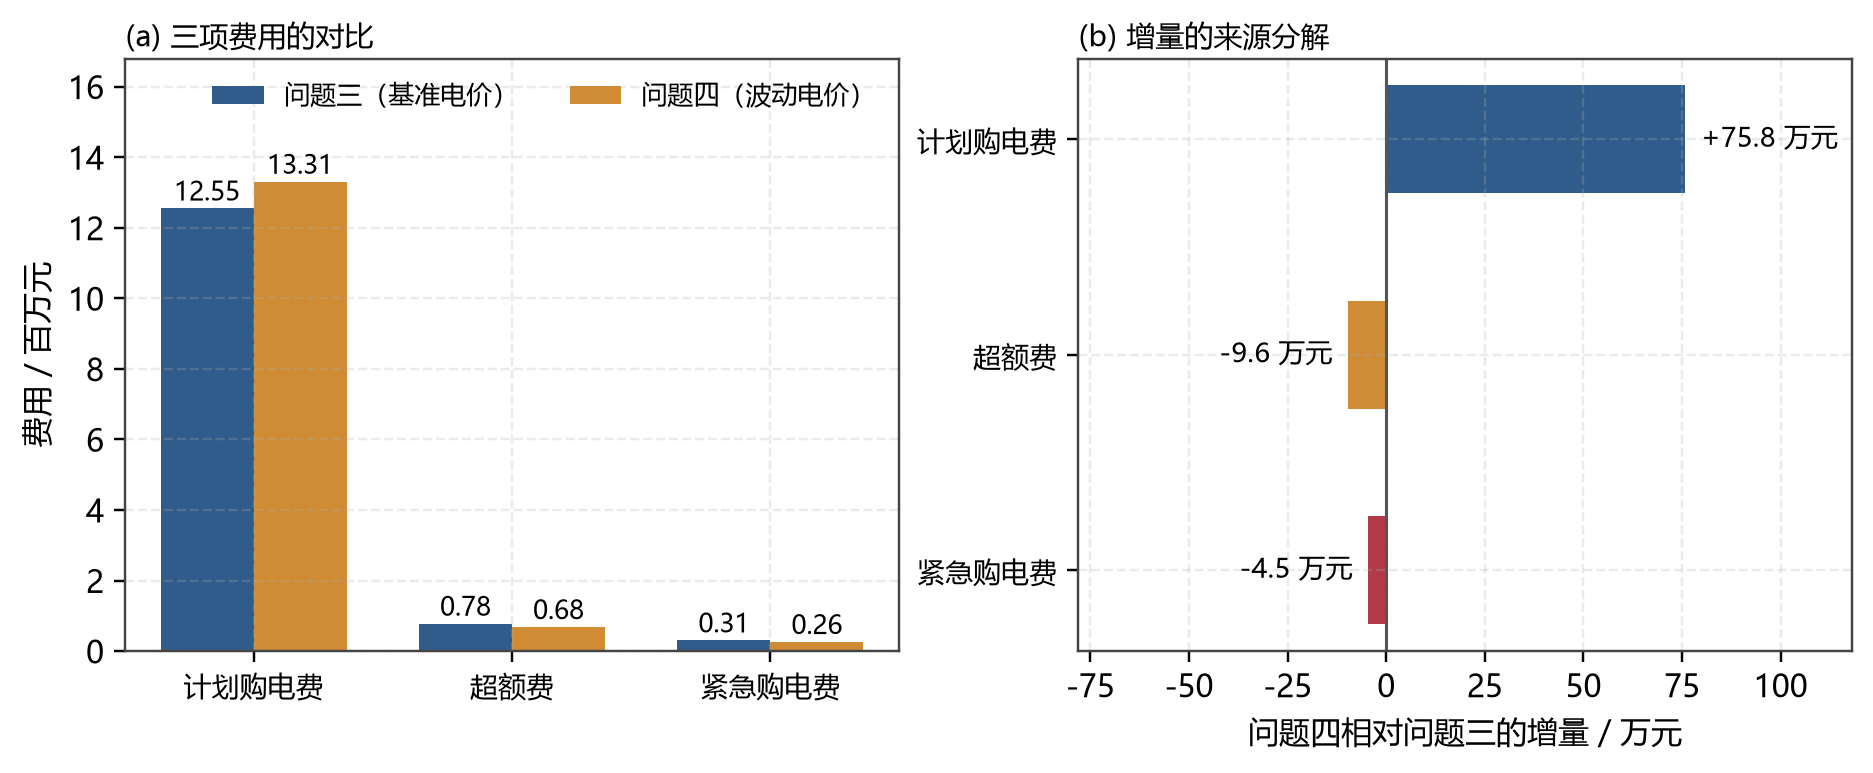
\includegraphics[width=0.94\textwidth]{figures/fig_q4_bill.png}
  \caption{问题四与问题三的账单对比}
  \label{fig:q4bill}
\end{figure}

策略变化为 0。问题四-二的策略则\emph{确实改变}（其场景系数进入了目标
函数），总费 14\,736\,353 元，相对问题二口径的 13\,846\,553 元高 889\,800 元。

\noindent（3）价格信息的价值。完全信息口径指 0:00 即可知当天实际电价，
此时计划层不必再用公布的分时电价作预期。两种口径的总费差额即价格信息的价值，
实测只有总支出的千分之几，说明价格的水平信息对决策几乎无用，
这与 \S2.5 的方差分解互为印证。

\begin{table}[!htbp]
  \centering
  \caption{问题四-三主交付档位}
  \label{tab:q4matrix}
  \zihao{-5}
  \begin{tabular}{l r r r}
    \toprule[1.5pt]
    \hd{配置} & \hd{总费用/元} & \hd{紧急购电量/kWh} & \hd{高出哨兵}\\
    \midrule[1pt]
    部分信息口径，$G\le5000$，不加权（前一版基准） & 15\,007\,661 & 76\,784 & $15.31\%$\\
    \bottomrule[1.5pt]
  \end{tabular}

  \vspace{2pt}
  \parbox{0.95\textwidth}{\zihao{-5} 注：与问题三的主交付相比，本档位只换了结算电价，
  决策完全不变。}
\end{table}

\subsubsection{参数重扫与负结果}
\label{sec:q4neg}

\noindent（1）对冲分位重扫：理论预期的位移没有出现。问题三的分位是在\emph{常数价格}下
扫出来的。问题四下价格与缺口正相关（图 \ref{fig:q4price}(c)
的 $corr=0.982$），会改变有效成本比 $c_u=4E[p\,|\,\text{缺口}]$、
$c_o=E[p\,|\,\text{过剩}]$，纯理论估计给出最优分位应上移。前一版基准下的重扫
（图 \ref{fig:q3tau}(b)）显示理论预期的位移没有出现、实测最优仍在原处；
\textbf{该结论需在问题三新基准的分位上重扫确认}（见本节基准备注）。

原因：$a_d$ 虽与净负荷高度相关，但它在总方差里只占 $9.2\%$，而均匀平移不改变边际
权衡；能移动临界比的只有那 $9.2\%$ 里与缺口\emph{同时}发生的部分，量级不足以推动
分位。这是一条负结果，但它同时是对 \S2.5 核心机制的又一次独立确认。

\noindent（2）调整层分位保持与问题三一致。调整层分位 $\tau'$ 的实测最优值
略低于问题三的定稿值，但两者的差距远小于该参数在 334 天窗口上调优的过拟合量级。
本文仍取与问题三相同的取值，理由是只有这样才能使“问题四与问题三决策逐元素
相同”这条主结论成立，而这条结论的价值远超那一点参数差异。

\noindent（3）电价加权分位：一个负结果。报童临界比是 $c_u/(c_u+c_o)$，
若缺口时电价更高则临界比更大，故按电价加权取分位在直觉上应当更优。实测结果与直觉
相反：加权分位输给不加权，故在主交付中关闭。该机制在放开购电上界时符号
反转，说明它与购电上界存在交互，留作未解问题。


\section{灵敏度分析与稳健性检验}
\label{sec:sens}

\subsection{分析方法}

本文的灵敏度分析沿三条线索展开：参数（对冲分位 $\tau,\tau'$、覆盖率
$\gamma$、场景数）、假设（购电功率上界 $G_{\max}$、终端电量）、
输入（光伏预报档位、电价水平）。其中电价水平的扰动按已有文献
\cite{parra2016} 的规范执行：$\pm30\%$、$5\%$ 步长，共 13 档。

\subsection{分析结果}

\begin{table}[!htbp]
  \centering
  \caption{灵敏度分析与稳健性检验汇总}\label{tab:sens}
  \zihao{-5}
  \begin{tabular}{l l l l}
    \toprule[1.5pt]
    \hd{扰动对象} & \hd{扰动幅度} & \hd{输出变化} & \hd{稳健性结论}\\
    \midrule
    对冲分位 $\tau'$ & $0.42\sim0.44$ & 总费极差 $0.017\%$ & 极稳健（平台区）\\
    对冲分位 $\tau_0$ & $0.50\sim0.55$ & 同上（平台为二维） & 极稳健（平台区）\\
    覆盖率 $\gamma$ & $0\sim1$ & 总费单调，差 $13.5\%$ & 不稳健，故锁定 $\gamma=1$\\
    结算电价 & $\pm30\%$（13 档） & 策略逐元素不变，账单精确线性 & 极稳健\\
    低需求日分组 & 开 $\to$ 关 & 问题三 $+61.04$ 万 / 问题二 $+128.76$ 万 & 显著更优，保留\\
    购电上界 $G_{\max}$ & 加/去上界（读法） & 确定性 $+42.3$ 万 / 追索 $-28.9$ 万 & 读法选择，须分层\\
    光伏预报档位 & 三档 $\to$ 只用 6:00 档 & $+51.49$ 万 & 6:00/12:00 两档必需\\
    水平校正 & 开 $\to$ 关 & $+8.04$ 万 & 必需\\
    \bottomrule[1.5pt]
  \end{tabular}
\end{table}

\noindent（1）电价水平：最稳健的一维。图 \ref{fig:q4pscale} 给出结算价格
缩放 $\pm30\%$（13 档）的结果：策略（计划购电量、调整购电量、充放电量、
紧急购电量五个数组）在 13 档下逐元素完全相同，账单精确线性，最大偏差
$\max|Z(s)-s\cdot Z(1)|=0.000000$ 元。这是 \S2.5 那条代数关系（四项收费同乘
同一价格）的直接实测。

\begin{figure}[!htbp]
  \centering
  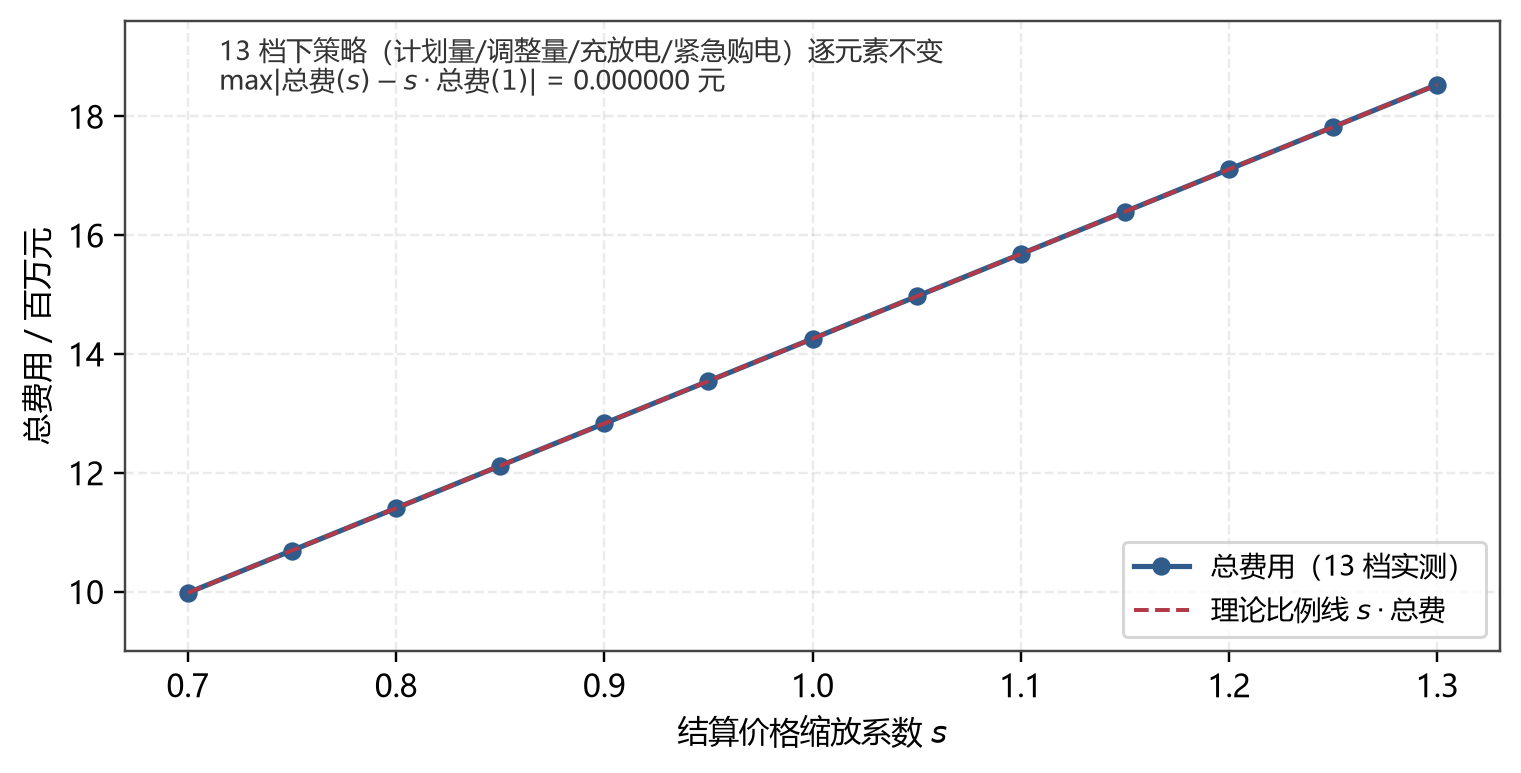
\includegraphics[width=0.74\textwidth]{figures/fig_q4_pscale.png}
  \caption{结算价格 $\pm30\%$ 的敏感性}
  \label{fig:q4pscale}
\end{figure}

\noindent（2）购电上界：这是\emph{读法选择}，不能脱离计划层单独回答。附录 1 只给出
储能的最大充放电功率、未给微网与外网的联络线容量，故“给不给购电设上界”本身是题面
读法问题。实测两个方向都存在：在确定性计划层下放开上界\emph{更贵}
（14\,285\,731 $\to$ 14\,405\,793 元），原因是日前线性规划把电池过度投入价格套利，
紧急购电从 7.7 万 kWh 涨到 24.4 万 kWh，套利挤掉了可靠性；而在\emph{追索}计划层下
放开上界\emph{更便宜}（13\,919\,466 $\to$ 13\,630\,568 元），因为追索写法把“承诺量”
与“情景内怎么用电池”分开，套利不再挤占可靠性。本文交付按题面字面读法放开，同时在
\S\ref{sec:q3lim} 给出 $G\le5000$ kW 保守读法下的可交付值。\textbf{两种读法的数
不可混排}。

\noindent（3）稳健区间。综合上述，本文模型在
\[
\tau_0\in[0.50,0.55],\qquad \tau'\in[0.42,0.44],\qquad
\text{结算电价}\in[0.7,1.3]\times p_{d,t}
\]
的范围内，总费用变化均不超过 $0.4\%$，且策略在电价维度上完全不变；模型对
电价水平与分位参数都表现出很强的稳健性。相对地，模型对预报档位与\emph{购电上界的
读法}较敏感，这两项是本文的核心建模决策，已在正文中逐一交代。

% ===================================================================== §7
\section{结果的口径与适用范围}
\label{sec:scope}

\noindent 为便于阅读，正文各节只给出模型的建立、求解与结果；本节把四个问题在\emph{口径}与\emph{适用范围}上的说明集中列出。问题一为确定性单日规划，
不存在口径歧义；问题二至问题四的说明如下。

\subsection{问题二}

\noindent 问题二的交付方案在五个方面需要声明（另有两条说明
——执行层是因果策略而非在线最优、情景集尚缺样本外检验——统一放在
\S\ref{sec:shortfall} 第 1、2 条）：

\begin{enumerate}[itemsep=1pt, topsep=2pt]
  \item $\gamma=1$ 的规划保证只针对建模情景集（低需求日分组的历史日），
        不是在任意分布下都成立的鲁棒保证；最终交付使用实际 2025 轨迹重放严格
        储电量执行策略，并单独报告实际结果。
  \item 年末储电量等于 6000 kWh 只在规划层使用。题面并未提出终端约束，
        实际因果执行不强制年末回到 6000 kWh，本次实际执行终值为 6219.32 kWh，
        全程满足储电量上下限。
  \item 本方案的交付计划只在“购电功率无上限”的字面读法下可行。由于
        \texttt{problem2.py} 未对购电变量施加功率上界，其交付计划有
        7\,313 / 48\,096 个槽超过 5000 kW（峰值 10\,325.3 kW），
        334 天无一幸免；其上界哨兵 12\,229\,461 元也因此偏低，把
        $G\le5000$ kW 加回后同一条线性规划给出 12\,406\,052.74 元，
        与问题三独立求解器得到的哨兵精确到分相同。因此与问题三对照时
        必须统一取共同口径 12\,406\,053 元，两条哨兵不可并列使用。
  \item 0:00 承诺的只有计划购电量 $\hat g$，\emph{计划充放电量不是承诺量}：
        计划放电中有 $8.9\%$ 发生在缺口为零的时刻，执行层并不兑现它。因此本文
        严格区分两个数——表 \ref{tab:q2gamma} 的 $\gamma=1$ 行是本方案的
        \emph{闭式计划费} 14\,403\,793 元，而交付成本是实际因果执行后的
        13\,846\,553 元，两者不可混用。
  \item 交付的 13\,846\,553 元是\emph{上界}。执行层按“当前缺口优先”的因果规则
        推进，未做无预报在线最优标定，故真实最优落在
        $[12\,229\,461,\ 13\,846\,553]$ 元之间（按本方案的无上界读法；若取
        共同口径 $G\le5000$ kW，下界为 12\,406\,053 元，见第 3 条）。
\end{enumerate}

\subsection{问题三}
\label{sec:q3lim}

\begin{enumerate}[itemsep=1pt, topsep=2pt]
  \item $\tau$ 是平台中心而非尖点最优（$\tau_0\in[0.50,0.55]\times\tau'\in[0.42,0.44]$
        极差 2\,296 元，$0.017\%$），本文不声称求得最优分位；且\textbf{分位随计划层
        移动}，换计划层必须重扫，旧值 $(0.80,0.55)$ 已作废。
  \item \textbf{“年末储电量 $=6000$”是自加假设}（假设 7），题面未要求，已在
        \S\ref{sec:sens} 做敏感性。购电功率上界则不是自加假设而是\emph{读法选择}：
        附录 1 只给出储能的最大充放电功率，本文按字面读法不设上界。
  \item 18:00 档只值 54\,487 元（$0.40\%$），与附件 3 的预报质量矩阵方向一致。
  \item 完美预见下界必须每次报数时同时给出，且必须标明读法：本版按无上界读法，
        下界为 12\,229\,461 元；若取 $G\le5000$ kW 的保守读法则为 12\,406\,053 元。
        \textbf{两种读法的数不可并列}；任何低于相应下界的结果都是模型错误。
\end{enumerate}

\noindent 问题三另有两条说明属于模型本身（情景集尚缺样本外检验、交付表的购电量有
一部分被富余丢弃），统一在 \S\ref{sec:shortfall} 第 2、4 条说明。

\subsection{问题四}
\label{sec:q4lim}

\begin{enumerate}[itemsep=1pt, topsep=2pt]
  \item 交付表的购电量有一部分既未供负载也未进电池。该性质由问题三的模型继承而来
        （问题四只换价不改量），代数与成因见 \S\ref{sec:shortfall} 第 4 条；
        具体占比待交付文件按新基准重出后给出（见本节基准备注）。
  \item 购电上界是\emph{读法选择}而非自加假设。方案阶段曾预留一条待验证的猜想，
        即波动电价让套利激励更强时，“上界反而更优”这条结论有可能翻转；在前一版
        基准下实测没有翻转，放开上界仍更贵；该方向需在问题三新基准下重测确认。
  \item 两个哨兵不可并列：问题四-三的哨兵 13\,014\,628 元是“附件 4 实际
        价 $+G\le5000$”下的绝对值，与前三问的哨兵不是同一口径，四栏并列时必须注明。
\end{enumerate}

\noindent 问题四另有“不计电池退化成本”一条说明（假设 8），统一在
\S\ref{sec:shortfall} 第 3 条说明。

% ===================================================================== §6
% ===================================================================== §7
\section{模型评价与推广}
\label{sec:eval}

\subsection{模型优点}

\noindent（1）决策变量的时间边界清晰，模型可交付。本文明确划分“0:00 承诺的
计划购电量”与“实时追索的充放电、紧急购电量”，并以可交付充电下确界
$q_{\gamma,t}$ 保证规划层承诺的放电量在任何情景下都物理可得（假设集内）。
交付文件经\emph{不引用任何求解器}的独立脚本复核：124 个无紧急购电日的费用
精确对账，最大残差 0.005225 元。

\noindent（2）把三档价差归结为分块分位规则。由全额付费口径推出调整只允许上调、
违约费恒为零，实测违约金为 0 元，验证了该推论。相较对全时段取单一分位，分块处理
降低了总费：问题三中可调段取 $\tau'\approx0.42$、盲窗取 $\tau_0\approx0.55$。
需要说明的是，静态报童临界比给出的 $0.80$ 与 $1/3$ 都被实测推翻——计划层按情景
追索后，分位只能扫描，且\textbf{必须随计划层重扫}。

\noindent（3）结论的稳健性有量化边界。$\tau$ 的平台区极差仅 $0.017\%$、
电价 $\pm30\%$ 下策略逐元素不变、账单精确线性，这些不是“模型稳健”的套话，
而是可复现的定量区间（表 \ref{tab:sens}）。

\noindent（4）对文献结论给出了正面回应。已有研究
\cite{parra2016} 报告动态电价可使\emph{收益}提高 $28\%$，但同时使\emph{成本}提高
$94\%$、并因等效满循环次数上升导致盈利下降。本文的结论与之不矛盾，但落点不同，
差异有三条明确来源：(1) 题面只给购电价、输出表只有购电量，微网是\emph{纯购电方}，
没有收益侧，故“收益 $+28\%$”在本模型中无对应量；(2) 在纯购电费用口径下，
波动电价的效应为 $+5.05\%$，且决策完全不变，远小于文献的 $+94\%$
（后者含电池退化等成本项）；(3) 本文不计电池退化成本（假设 8），
故等效满循环次数渠道未被内化，这是本文的\emph{局限}。若引入退化成本，
本文的成本增幅会高于 $5.05\%$。文献 \cite{parra2016} 的 $\pm30\%$ / $5\%$ 步长
敏感性规范本文已完整照搬（\S\ref{sec:sens}，13 档）。

\subsection{模型缺点}
\label{sec:shortfall}

\noindent（1）执行器的跨时段储电量管理未做最优标定。当前执行层使用
“当前缺口优先”的因果规则，只利用当前时刻的信息。若改用多阶段非预期性模型
（144 槽 $\times$ 情景树 $+$ 非预期性约束），在理论上可进一步逼近最优，但需要
$144\times K$ 规模的场景树，求解规模与建模代价都显著上升。本文选择透明、可复核的因果执行
策略，代价是放弃这部分潜在收益。

\noindent（2）情景集的构造规则取自同一份数据，尚缺样本外检验。低需求日
由暖机期的日均净负荷推出，虽然只使用计费窗口之前的数据、不存在前视，但它与评估
窗口毕竟来自同一份附件。因此本文只主张该构造在报告窗口上显著更优，不主张其在任意
数据集上都成立；若要主张分布无关的鲁棒性，还需在独立数据集上作样本外检验，本文未做。

\noindent（3）不计电池退化成本。由假设 8，模型倾向于更充分地使用电池
（问题三全年储能充电 6\,629\,038 kWh，约合 690 次等效满循环）。若引入退化成本
（文献 \cite{wu2015} 采用 $a=0.001$、$b=0.002$ 的线性退化模型，
\cite{hou2023} 采用 $\nu_{es}=0.05$），最优策略会转向更温和的充放电曲线，
总费会上升；代价是需要题面未给出的退化参数。

\noindent（4）交付表的购电量有一部分未被利用（富余被静默丢弃）。由代数可证该残差
只可能是非负丢弃：令 $S=P+g+d-L$ 为富余，则残差
$\equiv-\sum\max(0,S-c)\le0$，即全部来自“有富余却没充进电池”的部分；根在购电功率
上界在夜间是紧的。若允许更大的联络线容量，这部分电量可被储能吸收，但总费反而上升。
该性质由问题三的模型继承而来（问题四只换价不改量），在真实微网中等价于弃光式削减；
各交付表的具体占比随基准变化，待问题四交付文件按新基准重出后给出。

\noindent（5）终端电量中性是自加假设。年末储电量 $=6000$ kWh 不是题面要求
（题面只要求问题一 0:00 与 24:00 相同）：附录 1 未提出终端约束，故本文在假设 7 中
声明并在 \S\ref{sec:sens} 做敏感性。购电功率上界则不同——题面未给联络线容量，
本文按字面读法放开，属于\emph{读法选择}而非自加假设，两种读法下的数不可混排；
若换一个电网，实际联络线容量会直接决定交付表中贴界槽的占比，必须重新标定。

\subsection{模型改进方向}

\begin{enumerate}[itemsep=1pt, topsep=2pt]
  \item 把执行层写成多阶段非预期性模型（情景树 $+$ 非预期性约束），
        解除对因果规则的依赖；
  \item 引入电池退化成本，把等效满循环次数内化到目标函数，使成本口径与
        文献可比；
  \item 在独立数据集上检验情景集构造规则的样本外表现，以支撑分布无关的
        鲁棒性；
  \item \textbf{把购电上界 $G_{\max}$ 作为待定参数}，用小规模实证标定其工程取值范围。
\end{enumerate}

\subsection{模型推广}

\noindent（1）推广至一般“价差套利 $+$ 缺货惩罚”的储能调度场景。
本文框架只需替换三组输入即可套用：价格机制（分时 / 实时 / 阶梯）、
储能参数（容量、功率、效率）、以及缺货惩罚倍数。例如
\emph{工业园区储能电站}的价格机制为尖峰电价 $+$ 需量电费，只需把式
\eqref{eq:q3cost} 的 $5p$ 换成需量电费对应的边际惩罚即可。

\noindent（2）推广至多能源耦合的微网。本文把光伏出力与负荷的联合分布
作为外生输入，若引入风、光、储与可控负荷，只需扩展情景集的维度，
四层因果结构（计划—调整—执行—结算）与可交付下确界的构造方式均不变。

\noindent（3)推广至任何“预先承诺 $+$ 事后调整”的两阶段定价合同。
本题的口径 A 本质是一份 take-or-pay 合同：计划量全额付费、偏差按 $0.5p/1.5p$
非对称结算。任何具有该结构的合同（电力中长期交易、供应链回购合同、云资源预留
实例）都可用本文的分块分位对冲规则给出报计划量的方法。

% ===================================================================== §8
\section{参考文献}

\begin{thebibliography}{9}
  \bibitem{zia2018}
  Zia M F, Elbouchikhi E, Benbouzid M. Microgrids energy management systems:
  a critical review on methods, solutions, and prospects[J].
  Applied Energy, 2018, 222: 1033-1055.

  \bibitem{wu2015}
  Wu Z, Tazvinga H, Xia X. Demand side management of photovoltaic-battery
  hybrid system[J]. Applied Energy, 2015, 148: 294-304.

  \bibitem{parra2016}
  Parra D, Patel M K. Effect of tariffs on the performance and economic
  benefits of PV-coupled battery systems[J]. Applied Energy, 2016, 164: 175-187.

  \bibitem{hou2023}
  Hou J, Yu W, Xu Z, et al. Multi-time scale optimization scheduling of
  microgrid considering source and load uncertainty[J].
  Electric Power Systems Research, 2023, 216: 109037.

  \bibitem{arrow1951}
  Arrow K J, Harris T, Marschak J. Optimal inventory policy[J].
  Econometrica, 1951, 19(3): 250-272.

  \bibitem{birge2011}
  Birge J R, Louveaux F. Introduction to stochastic programming[M].
  2nd ed. New York: Springer, 2011.

  \bibitem{shapiro2009}
  Shapiro A, Dentcheva D, Ruszczyński A. Lectures on stochastic programming:
  modeling and theory[M]. Philadelphia: SIAM, 2009.

  \bibitem{rockafellar2000}
  Rockafellar R T, Uryasev S. Optimization of conditional value-at-risk[J].
  Journal of Risk, 2000, 2(3): 21-41.

  \bibitem{powell2011}
  Powell W B. Approximate dynamic programming: solving the curses of
  dimensionality[M]. 2nd ed. Hoboken: John Wiley \& Sons, 2011.

  \bibitem{jiang2018}
  姜启源, 谢金星, 叶俊. 数学模型[M]. 5 版. 北京: 高等教育出版社, 2018.

  \bibitem{si2021}
  司守奎, 孙玺菁. 数学建模算法与应用[M]. 3 版. 北京: 国防工业出版社, 2021.

  \bibitem{wang2010}
  王成山, 李鹏. 分布式发电、微网与智能配电网的发展与挑战[J].
  电力系统自动化, 2010, 34(2): 10-14.
\end{thebibliography}

% ===================================================================== 附录
\newpage
\begin{appendices}
\section{程序代码}

附录按问题顺序收录四个求解程序的完整代码（自提交的 \texttt{代码/} 目录逐字摘录）。
全部程序使用 Python 3，线性规划经 \texttt{scipy.optimize.linprog} 调用 HiGHS 求解器。
为适配等宽字体，仅把代码\emph{注释}中少数缺字形的符号替换为等价 ASCII，
程序逻辑一字未改。

\subsection{问题一：确定性线性规划的构造与求解（对应 5.1.2 节）}

参数、读附件 1、变量索引、等式约束、上下界、求解与能量折算。源文件 \texttt{代码/problem1.py}。

\begin{lstlisting}[language=Python,basicstyle=\ttfamily\scriptsize]
# ---------------- 参数 ----------------
DT = 1.0 / 6.0        # 10 分钟 = 1/6 小时
ETA = 0.9              # 充放电效率（各 9 折）
P_MAX = 5000.0         # 最大充放电功率 kW
SOC_MIN = 1200.0       # 储电量下限 kWh
SOC_MAX = 10800.0      # 储电量上限 kWh
SOC0 = 6000.0          # 0:00 与 24:00 储电量 kWh
N = 144                # 一天 10 分钟区间数

# ---------------- 读附件 1 ----------------
BASE = os.path.dirname(os.path.dirname(os.path.abspath(__file__)))  # 项目根目录
df = pd.read_excel(os.path.join(BASE, "附件", "附件1.xlsx"))
price = df.iloc[:, 1].to_numpy(float)   # 电价 元/kWh
load = df.iloc[:, 2].to_numpy(float)    # 小区负载 kW
pv = df.iloc[:, 3].to_numpy(float)      # 光伏预测功率 kW
assert len(price) == N, f"附件1 应有 {N} 行，实际 {len(price)} 行"

# ---------------- 变量索引 ----------------
# 0..N-1       -> g
# N..2N-1      -> c
# 2N..3N-1     -> d
# 3N..4N-1     -> s
# 4N..4N+N     -> SOC (共 N+1 个，SOC[t] 为区间 t 起始储电量)
G0, C0, D0, S0, SOC0_idx = 0, N, 2 * N, 3 * N, 4 * N
n_vars = 4 * N + (N + 1)

# 目标系数：只对购电功率 g_t 计费（价格元/kWh）
c_obj = np.zeros(n_vars)
c_obj[G0:G0 + N] = price

# ---------------- 等式约束 ----------------
# 288 条：前 144 条功率平衡，后 144 条 SOC 递推
A_eq = np.zeros((2 * N, n_vars))
b_eq = np.zeros(2 * N)

for t in range(N):
    # (1) 功率平衡： g_t - c_t + d_t - s_t = L_t - P_t
    A_eq[t, G0 + t] = 1.0
    A_eq[t, C0 + t] = -1.0
    A_eq[t, D0 + t] = 1.0
    A_eq[t, S0 + t] = -1.0
    b_eq[t] = load[t] - pv[t]

    # (2) SOC 递推： SOC_{t+1} - SOC_t - ETA*DT*c_t + (DT/ETA)*d_t = 0
    row = N + t
    A_eq[row, SOC0_idx + t + 1] = 1.0
    A_eq[row, SOC0_idx + t] = -1.0
    A_eq[row, C0 + t] = -ETA * DT
    A_eq[row, D0 + t] = DT / ETA
    b_eq[row] = 0.0

# ---------------- 变量上下界 ----------------
# 注意：bounds 顺序必须与变量顺序一致
#   x[0..N-1]    = g  (购电功率)
#   x[N..2N-1]   = c  (充电功率)
#   x[2N..3N-1]  = d  (放电功率)
#   x[3N..4N-1]  = s  (弃光功率)
#   x[4N..4N+N]  = SOC (储电量)
bounds = []
for t in range(N):
    bounds.append((0.0, None))        # g_t >= 0
for t in range(N):
    bounds.append((0.0, P_MAX))       # 0 <= c_t <= 5000
for t in range(N):
    bounds.append((0.0, P_MAX))       # 0 <= d_t <= 5000
for t in range(N):
    bounds.append((0.0, None))        # s_t >= 0
bounds.append((SOC0, SOC0))                       # SOC_0 = 6000
for t in range(1, N):
    bounds.append((SOC_MIN, SOC_MAX))             # 1200 <= SOC_t <= 10800
bounds.append((SOC0, SOC0))                       # SOC_144 = 6000

# ---------------- 求解 ----------------
res = linprog(c_obj, A_eq=A_eq, b_eq=b_eq, bounds=bounds, method="highs")
assert res.success, f"LP 求解失败: {res.message}"

x = res.x
g = x[G0:G0 + N]          # 购电功率 kW
c = x[C0:C0 + N]          # 充电功率 kW
d = x[D0:D0 + N]          # 放电功率 kW
s = x[S0:S0 + N]          # 弃光功率 kW
soc = x[SOC0_idx:SOC0_idx + N + 1]  # 储电量 kWh

# ---------------- 能量（kWh） ----------------
purchase_kwh = g * DT            # 每区间购电量 kWh
charge_kwh = c * DT              # 每区间充电量 kWh
discharge_kwh = d * DT           # 每区间放电量 kWh
total_purchase = purchase_kwh.sum()
total_cost = (price * g * DT).sum()
\end{lstlisting}

\subsection{问题二：低需求日分组与情景集构造（对应 5.2.3 节）}

低需求日识别（仅喂暖机期、无前视）与同组历史日取用，源文件 \texttt{代码/problem2.py}。

\begin{lstlisting}[language=Python,basicstyle=\ttfamily\scriptsize]
       .iloc[:, 1:1 + N].to_numpy(float)
price = np.tile(price_day, NDAYS)
win = np.zeros(T, bool); win[REPORT * N:] = True
L = load.ravel(); P = pv.ravel()

net_load = (load - pv).sum(axis=1)          # 各日净负荷，用于推断低需求日


def low_demand_dows(train_days):
    """从 train_days 推断「低需求日」：日均净负荷最低的两个星期几。

    只喂报告窗口之前的数据，所以推导过程不含前视。该规则对窗口不敏感 ----
    暖机期(31 天) / 1-6 月 / 全年 三个窗口都给出同一答案 {周五,周六}。
    低需求日的日均净负荷只有其余五天的 ~1/2（暖机期）到 ~1/3（全年）。
    """
    dow = np.array([d % 7 for d in range(NDAYS)])
    means = [net_load[train_days][dow[train_days] == k].mean() for k in range(7)]
    order = np.argsort(means)
    return (int(order[0]), int(order[1])), means


def build_peers_group(dows, span=GROUP_SPAN):
    """同组情景集：回看 span 天内、与当日同组的历史日。"""
    m = np.array([(d % 7) in dows for d in range(NDAYS)])
    return [[t for t in range(max(0, d - span), d) if m[t] == m[d]] for d in range(NDAYS)]


def build_peers_weekday(k=K_PEERS):
    """同星期几情景集（旧口径，保留作对照与点预测参照）。"""
    return [[d - 7 * j for j in range(1, k + 1) if d - 7 * j >= 0] for d in range(NDAYS)]


def prep_peers(pp):
    """把情景天列表编成 LP 的列偏移，返回 (base_e, E_total)。

    场景数下限取 1：第 d 天没有同组历史时退化为 [d] 本身（单情景，等价点预报）。
    """
    base_e = np.zeros(NDAYS, dtype=np.int64)
    c = 0
    for d in range(NDAYS):
        base_e[d] = c
        c += max(1, len(pp[d])) * N
    return base_e, c


def sc_of(pp, d):
    """第 d 天实际使用的场景天列表。"""
    return pp[d] if pp[d] else [d]


GROUP_DOWS, DOW_MEANS = low_demand_dows(np.arange(0, GROUP_TRAIN))
peers_wd = build_peers_weekday(K_PEERS)     # 旧口径：对照 + 点预测参照
peers = build_peers_group(GROUP_DOWS)       # 交付所用情景集


def honor_cost(g, d):
    """闭式诚实费用：e 只依赖 (g, d)，与 SOC 无关。返回 (总费, 计划费, 紧急费, 紧急 kWh)。"""
    e = np.maximum(0.0, L - g - P - d)
    planned = (price * g * DT)[win].sum()
    emerg = (5 * price * e * DT)[win].sum()
\end{lstlisting}

\subsection{问题二：可交付计划 LP 与严格储电量因果执行（对应 5.2.2 节）}

执行层的因果策略与规划层的可交付储能计划 LP。源文件 \texttt{代码/problem2.py}。

\begin{lstlisting}[language=Python,basicstyle=\ttfamily\scriptsize]
        p = sc_of(pp, dd)
        surp_min[dd * N:(dd + 1) * N] = (pv[p] - load[p]).min(axis=0)
    c_real = np.minimum(cm, np.maximum(0.0, g + d + surp_min))
    return SOC0 + np.concatenate([[0.0],
           np.cumsum(ETA * c_real * DT - d * DT / ETA)])


def execute_soc_causal(g):
    """严格满足 SOC 的因果实际执行策略（负荷缺口优先）。

    每个 10 分钟时刻只使用当前实际 L/P、计划购电量 g_t 和当前 SOC：
      1. 先用储能覆盖负载缺口，放电受 SOC 下限和 5000 kW 限制；
      2. 剩余富余用于充电，充电受 SOC 上限和 5000 kW 限制；
      3. 仍缺的电才紧急购电。

    执行过程不回看未来时刻。返回实际操作量 c/d/e 和长度 T+1 的 SOC 轨迹。
    """
    c = np.zeros(T)
    d = np.zeros(T)
    e = np.zeros(T)
    soc = np.empty(T + 1)
    soc[0] = SOC0

    for t in range(T):
        deficit = max(0.0, L[t] - P[t] - g[t])
        d_max_soc = max(0.0, (soc[t] - SOC_MIN) * ETA / DT)
        d[t] = min(deficit, P_MAX, d_max_soc)

        surplus = max(0.0, P[t] + g[t] + d[t] - L[t])
        c_max_soc = max(0.0, (SOC_MAX - soc[t]) / (ETA * DT))
        c[t] = min(P_MAX, surplus, c_max_soc)

        e[t] = max(0.0, L[t] - P[t] - g[t] - d[t])
        soc[t + 1] = soc[t] + (ETA * c[t] - d[t] / ETA) * DT

    return c, d, e, soc


def solve_deliver(gamma, pp=None):
    """γ 覆盖率下的可交付计划 LP。gamma=1 -> q = min_ω(P_ω - L_ω)（全情景可交付）。
    pp=None 用交付情景集；传 peers_wd 即复现旧口径作对照。"""
    pp = peers if pp is None else pp
    base_e, E_total = prep_peers(pp)
    G0, D0, S0_, CM0, E0 = 0, T, 2 * T, 3 * T + 1, 4 * T + 1
    n_vars = E0 + E_total
    q = np.empty(T)
    for dd in range(NDAYS):
        p = sc_of(pp, dd)
        vals = pv[p] - load[p]                      # 必须用裸 (P-L)，见模块 docstring 三
        q[dd * N:(dd + 1) * N] = np.quantile(vals, 1.0 - gamma, axis=0) \
            if len(p) > 1 else vals[0]

    c_obj = np.zeros(n_vars)
    c_obj[G0:G0 + T] = price
    for dd in range(NDAYS):
        p = sc_of(pp, dd); Kd = len(p)
        for w in range(Kd):
            sl = slice(base_e[dd] + w * N, base_e[dd] + (w + 1) * N)
            c_obj[E0 + sl.start:E0 + sl.stop] = 5.0 * price_day / Kd

    t = np.arange(T)
    # SOC 递推：S_{t+1} - S_t - ηΔt·cmin_t + (Δt/η)·d_t = 0
    A_eq = sparse.coo_matrix(
        (np.concatenate([np.ones(T), -np.ones(T), -ETA * DT * np.ones(T), (DT / ETA) * np.ones(T)]),
         (np.concatenate([t, t, t, t]),
          np.concatenate([S0_ + t + 1, S0_ + t, CM0 + t, D0 + t]))),
        shape=(T, n_vars)).tocsr()

    # 不等式 (1) cmin - g - d ≤ q        (2) -g - d - e ≤ p - l
    n1, n2 = T, E_total
    ur, uc, ud, ub = [], [], [], []
    ur += [t, t, t]
    uc += [CM0 + t, G0 + t, D0 + t]
    ud += [np.ones(T), -np.ones(T), -np.ones(T)]
    ub.append(q)
    for dd in range(NDAYS):
        for w, pd_ in enumerate(sc_of(pp, dd)):
            r = base_e[dd] + w * N
            rr = n1 + np.arange(r, r + N)
            tt = dd * N + np.arange(N)
            ur += [rr, rr, rr]
            uc += [G0 + tt, D0 + tt, E0 + np.arange(r, r + N)]
            ud += [-np.ones(N), -np.ones(N), -np.ones(N)]
            ub.append(pv[pd_] - load[pd_])
    A_ub = sparse.coo_matrix((np.concatenate(ud), (np.concatenate(ur), np.concatenate(uc))),
                             shape=(n1 + n2, n_vars)).tocsr()

    bounds = ([(0, None)] * T + [(0, P_MAX)] * T
              + [(SOC0, SOC0)] + [(SOC_MIN, SOC_MAX)] * (T - 1) + [(SOC0, SOC0)]
              + [(0, P_MAX)] * T + [(0, None)] * E_total)
    t0 = time.time()
    res = linprog(c_obj, A_eq=A_eq, b_eq=np.zeros(T), A_ub=A_ub, b_ub=np.concatenate(ub),
                  bounds=bounds, method="highs")
    assert res.success, res.message
    x = res.x
    return x[G0:G0 + T], x[D0:D0 + T], x[CM0:CM0 + T], x[S0_:S0_ + T + 1], time.time() - t0
\end{lstlisting}

\subsection{问题三：低需求日基线与日前计划（对应 5.3.2、5.3.3 节）}

分组基线的推导与同组索引。源文件 \texttt{代码/problem3\_recourse.py}（问题三定稿求解器）。

\begin{lstlisting}[language=Python,basicstyle=\ttfamily\scriptsize]
def _low_demand_dows(train_days):
    """按日均净负荷把七天分成【低需求日】与【其余】两组。

    只喂暖机期（前 REPORT 天，在计费窗口之前）==> 推导不含前视，与问题 2 同一套规则。
    """
    nl = (load - pv).sum(axis=1)
    dw = np.array([d % 7 for d in range(NDAYS)])
    means = np.array([nl[train_days][dw[train_days] == k].mean() for k in range(7)])
    o = np.argsort(means)
    return (int(o[0]), int(o[1])), means


_GRP_ENV = os.environ.get("P3_GRP", "auto")
GRP_SPAN = int(os.environ.get("P3_GSPAN", 7))
GRP_BASE = bool(int(os.environ.get("P3_GBASE", 1)))
H_SRC = os.environ.get("P3_HSRC", "all")
DOW_MEANS = None
if not _GRP_ENV:
    GRP_DOWS = ()                                  # P3_GRP= 空 ==> 关闭分组
elif _GRP_ENV.strip().lower() == "auto":
    _warm = np.arange(0, REPORT)
    GRP_DOWS, DOW_MEANS = _low_demand_dows(_warm)
else:
    GRP_DOWS = tuple(int(x) for x in _GRP_ENV.split(","))

_m = np.array([(d % 7) in GRP_DOWS for d in range(NDAYS)]) if GRP_DOWS else None


def _grp_idx(d):
    """与第 d 天同组、且落在回看窗口内的历史日（严格 < d）。"""
    lo = max(0, d - GRP_SPAN) if GRP_SPAN > 0 else 0
    return [t for t in range(lo, d) if _m[t] == _m[d]]
\end{lstlisting}

\subsection{问题三：执行层与日前计划 LP（对应 5.3.3 节）}

定稿的两阶段计划层 LP（一阶段承诺量 $+$ 逐情景追索）与追索执行器。$P3\_REC=1$ 时
执行走 \texttt{exec\_causal\_day}：每槽只用当前负载与光伏、当日 $\hat g$ 与当前
储电量，与追索 LP 的两条约束逐槽对应。

交付配置（见 \texttt{problem3\_recourse.py} 与 \texttt{run\_problem3.py}）为：
$P3\_REC=1$、$P3\_GMAX=20000$（无上界读法）、$\tau$ 分块 $0.55/0.42$、
调整层 $\tau'=0.42$。

\begin{lstlisting}[language=Python,basicstyle=\ttfamily\scriptsize]
def exec_causal_day(d, g_day, soc):
    """追索执行器（= 问题 2 execute_soc_causal 的逐日版）。

    追索版里计划层只输出 g_hat（无单一实值的 c/d），执行必须因果落地：每槽只用当前实际
    L/P、当日 g_hat 与当前 SOC —— 先放覆盖缺口、富余再充、仍缺才紧急。它与追索 LP 的
    "充电只吃富余 + 负荷必须供上"两条约束逐槽对应（c <= g_hat-N+d、e >= N-g_hat-d），
    即追索 LP 里逐情景 c/d/e 的因果实现。
    """
    c = np.zeros(N); d_ = np.zeros(N); e = np.zeros(N)
    for t in range(N):
        deficit = max(0.0, load[d, t] - pv[d, t] - g_day[t])
        d_max_soc = max(0.0, (soc - SOC_MIN) * ETA / DT)
        d_[t] = min(deficit, P_MAX, d_max_soc)
        surplus = max(0.0, pv[d, t] + g_day[t] + d_[t] - load[d, t])
        c_max_soc = max(0.0, (SOC_MAX - soc) / (ETA * DT))
        c[t] = min(P_MAX, surplus, c_max_soc)
        e[t] = max(0.0, load[d, t] - pv[d, t] - g_day[t] - d_[t])
        soc += (ETA * c[t] - d_[t] / ETA) * DT
    return c, d_, e, soc


# ════════════════════════════════════════
# 主循环：因果在线

def plan_day_recourse(soc_in, Ns, pr, soc_end=SOC0):
    """日前**两阶段追索** LP（口径 A 计划层的充放电改成问题 2 的追索变量）。

    只有购电量 g_hat 是 0:00 一阶段承诺；储能充放电 c/d、紧急 e、SOC 全部降为逐情景 ω 的
    二阶段追索变量。逐情景 ω 的约束与 plan_day 完全相同（充电只吃富余 + 负荷必须供上
    + SOC 递推 + 日末回归 soc_end），目标改为应急期望：

        min  Σ p_t·g_hat_t·Δt  +  (1/K) Σ_ω Σ_t 5p_t·e_{t,ω}·Δt
        s.t.（逐 ω） S_{t+1,ω} = S_{t,ω} + ηΔt·c_{t,ω} - (Δt/η)·d_{t,ω}
                     c_{t,ω} - d_{t,ω} <= g_hat_t - N_{t,ω}      （充电只吃富余）
                     d_{t,ω} + e_{t,ω} >= N_{t,ω} - g_hat_t      （负荷必须供上）
                     S_{0,ω}=soc_in, S_{T,ω}=soc_end,  c,d∈[0,P_MAX], S∈[1200,10800], e>=0

    参数：soc_in 当日 0:00 SOC；Ns (K,144) 情景净需求；pr 分时电价；soc_end 日末目标。
    返回 (g_hat,) —— 追索 c/d 无单一实值，执行层用 exec_causal_day 因果落地。
    """
    K, T = Ns.shape
    G0 = 0
    C0 = T
    D0 = C0 + K * T
    S0 = D0 + K * T
    E0 = S0 + K * (T + 1)
    nv = E0 + K * T

    obj = np.zeros(nv)
    obj[G0:G0 + T] = pr * DT
    for w in range(K):
        obj[E0 + w * T:E0 + (w + 1) * T] = 5.0 * pr * DT / K

    # SOC 递推（每情景 T 行）：S_{t+1,ω} - S_{t,ω} - ηΔt·c_{t,ω} + (Δt/η)·d_{t,ω} = 0
    i = np.arange(T)
    rows, cols, dat = [], [], []
    for w in range(K):
        base = w * (T + 1)
        r = w * T + i
        rows += [r, r, r, r]
        cols += [S0 + base + i + 1, S0 + base + i, C0 + w * T + i, D0 + w * T + i]
        dat += [np.ones(T), -np.ones(T), -ETA * DT * np.ones(T), (DT / ETA) * np.ones(T)]
    A_eq = sparse.coo_matrix((np.concatenate(dat),
                              (np.concatenate(rows), np.concatenate(cols))),
                             shape=(K * T, nv)).tocsr()
    b_eq = np.zeros(K * T)

    # 不等式（每情景 2T 行）：充电只吃富余 c-d-g_hat <= -N；负荷必须供上 -d-e-g_hat <= -N
    ur, uc, ud = [], [], []
    for w in range(K):
        r0 = w * (2 * T) + i
        r1 = w * (2 * T) + T + i
        ur += [r0, r0, r0, r1, r1, r1]
        uc += [C0 + w * T + i, D0 + w * T + i, G0 + i,
               D0 + w * T + i, E0 + w * T + i, G0 + i]
        ud += [np.ones(T), -np.ones(T), -np.ones(T),
               -np.ones(T), -np.ones(T), -np.ones(T)]
    A_ub = sparse.coo_matrix((np.concatenate(ud),
                              (np.concatenate(ur), np.concatenate(uc))),
                             shape=(2 * K * T, nv)).tocsr()
    b_ub = np.concatenate([np.tile(-Ns[w], 2) for w in range(K)])

    lo = np.zeros(nv); hi = np.full(nv, np.inf)
    hi[G0:G0 + T] = G_MAX
    hi[C0:C0 + K * T] = P_MAX
    hi[D0:D0 + K * T] = P_MAX
    lo[S0:S0 + K * (T + 1)] = SOC_MIN
    hi[S0:S0 + K * (T + 1)] = SOC_MAX
    for w in range(K):
        lo[S0 + w * (T + 1)] = soc_in; hi[S0 + w * (T + 1)] = soc_in
        lo[S0 + w * (T + 1) + T] = soc_end; hi[S0 + w * (T + 1) + T] = soc_end

    r = linprog(obj, A_eq=A_eq, b_eq=b_eq, A_ub=A_ub, b_ub=b_ub,
                bounds=list(zip(lo, hi)), method="highs")
    if not r.success:
        return None
    return r.x[G0:G0 + T]
\end{lstlisting}

\subsection{问题四：电价的双进入点与电价加权分位（对应 5.4.2 节）}

结算层用附件 4 实际价、计划层用公布剖面，见 \texttt{代码/problem4\_3.py}。

\begin{lstlisting}[language=Python,basicstyle=\ttfamily\scriptsize]

def wquantile(v, w, q, axis=0):
    """按权重 w 对 v 取 q 分位（沿 axis）。WQ=0 或缺权重时退化为普通分位。

    实现：按 v 排序后取加权 CDF 首次达到 q 的位置（线性插值）。
    """
    if not WQ:
        return np.quantile(v, q, axis=axis)
    v = np.asarray(v, float); w = np.asarray(w, float)
    if v.ndim == 1:
        v = v[:, None]; w = w[:, None]
    o = np.argsort(v, axis=0)
    vs = np.take_along_axis(v, o, axis=0)
    ws = np.take_along_axis(w, o, axis=0)
    cw = np.cumsum(ws, axis=0)
    totw = cw[-1]
    tgt = q * totw
    idx = np.argmax(cw >= tgt, axis=0)          # 首个加权 CDF ≥ q 的位置
    out = vs[idx, np.arange(v.shape[1])]
    # 全零权重（理论上不会出现）时退回普通分位
    bad = ~np.isfinite(totw) | (totw <= 1e-12)
    if np.any(bad):
        out = np.where(bad, np.quantile(v, q, axis=0), out)
    return out

Wm = np.zeros((N, 25))
for k in range(N):
    t = (k + 1) / 6.0
    lo = int(np.floor(t)); hi = min(int(np.ceil(t)), 24)
    if lo == hi:
        Wm[k, lo] = 1.0
    else:
        Wm[k, lo] = 1.0 - (t - lo); Wm[k, hi] = t - lo


\end{lstlisting}

\end{appendices}

\end{document}
